%%%%%%%%%%%%%%%%%%%%%%%%%%%%%%%%%%%%%%%%%%%%%%%%%%%%%%%%%%%%%%%%%%
% The following comments were written in Portuguese, because this 
% template applies only for School of Technology at University 
% of Campinas, Brazil.
%
% Este é um modelo Latex para monografias de Trabalhos de Conclusão 
% de Curso (TCC) na graduação, monografias de Mestrado e Teses de 
% doutorado da Faculdade de Tecnologia (FT) da Universidade 
% Estadual de Campinas (UNICAMP).
%
% Esse modelo e seu respectivo arquivo de classe de documento 
% foram adaptado do modelo de teses e dissertações do 
% Instituto de Computação da UNICAMP e estão de acordo com a 
% Norma CPG 001/2019.
%
% Autor: André Leon Sampaio Gradvohl, Dr.
% Email:     gradvohl@ft.unicamp.br
% Lattes CV: http://lattes.cnpq.br/9343261628675642
% ORCID:     0000-0002-6520-9740
% 
% Última versão: 14/junho/2020
%
% Adições/Alterações nesta última versão:
% - Adição de informações sobre a inclusão do arquivo com a 
%   ficha catalográfica ou página em branco.
% - Ajustes no idioma para a lista de abreviações e siglas.
% - Adequações na lista de símbolos.
% - Inclusão do pacote silence para suprimir os "warnings" 
%   referentes à inclusão do arquivo "brazilian-abnt". 
% - Adição da opção "noFig" para acelerar a compilação, sem 
%   a adição de figuras. Use apenas junto com a opção Draft.
% - Adição de comandos para referenciar múltiplos capítulos, 
%   seções, figuras, tabelas, equações.
% - Adição de citação a software na bibliografia.
%%%%%%%%%%%%%%%%%%%%%%%%%%%%%%%%%%%%%%%%%%%%%%%%%%%%%%%%%%%%%%%%%%
%
% Para a versão final do texto, acrescente a palavra "Final".
\documentclass[Portugues,Draft]{tese-FT}

\addbibresource{bibliografia.bib}

\begin{document}

\autor{Gabriel Domingues Ferreira}

\titulo{RASTREAMENTO DE EXPOSIÇÃO À DOENÇAS INFECCIOSAS POR APLICATIVO CELULAR}

\orientador{Prof. Dr. Plínio Roberto Souza Vilela}

\bsi

% Defina a data da defesa no formato {Dia}{Mês}{Ano}
% Use apenas números! O template transformará em palavras,
% se necessário.
\datadadefesa{12}{6}{2020}

% Para a versão final defina:
% Repita o nome do Orientador(a) no primeiro avaliador
\avaliadorA{Prof. Dr. Plínio Roberto Souza Vilela}{FT/UNICAMP}
\avaliadorB{Profa. Dra. Segunda Avaliadora}{Instituição da segunda avaliadora}
\avaliadorC{Dr. Terceiro Avaliador}{Instituição do terceiro avaliador}

% Para incluir a ficha catalográfica em PDF na versão final, 
% copie o arquivo PDF para o projeto no Overleaf, descomente 
% e informe o nome do arquivo no comando a seguir.
% \fichacatalografica{SeuArquivo.pdf}
%
% Para deixar uma página em branco no lugar da ficha 
% catalográfica
\fichacatalografica{branco.pdf} % Português

\paginasiniciais

% Se houver epígrafe, descomente e edite as linhas a seguir:
% \begin{epigrafe}
% {\it
% Vita brevis,\\
% ars longa,\\
% occasio praeceps,\\
% experimentum periculosum,\\
% iudicium difficile.}
%
% \hfill (Hippocrates)
% \end{epigrafe}

% Adicione no arquivo "agradecimentos.tex" os seus agradecimentos
% Caso prefira omitir os agradecimentos, comente a linha a seguir.
% \prefacesection{Agradecimentos}
Coloque nesse arquivo os agradecimentos àqueles que o ajudaram no seu trabalho. Os agradecimentos devem ocupar uma única página. Não esqueça de adicionar a frase a seguir.

O presente trabalho foi realizado com apoio da Coordenação de Aperfeiçoamento de Pessoal de Nível Superior -- Brasil (CAPES) -- Código de Financiamento 001.

% Sempre deve haver um resumo em português:
\begin{resumo}
O início do ano de 2020 foi marcado pela pandemia causada pelo coronavírus, e por conta disso, diversos países perceberam as ameaças que doenças infecciosas podem trazer à humanidade e voltaram suas atenções para combater sua transmissão. 
Uma das soluções para diminuir a alta taxa de transmissão da doença foi o rastreamento de contatos. Esse rastreamento acontece da seguinte forma: no momento que uma pessoa é diagnosticada como infectada, ela deve responder algumas perguntas sobre quem ela se encontrou nos últimos dias. As pessoas que forem rastreadas a partir dessas perguntas devem se isolar mesmo que não estejam apresentando sintomas, para impedir que o vírus continue se espalhando.

Essa é uma maneira pouco eficiente de rastreamento por dois principais motivos: o primeiro é que é totalmente manual, isso reflete na necessidade de muitos recursos humanos serem alocados para entrevistar os infectados, fazer ligações, envio de e-mails e mensagens para as pessoas que tiveram contato com ele. E quanto mais recursos envolvidos nesse processo, mais caro ele se torna. O segundo motivo é que o rastreamento depende inteiramente das lembranças do indivíduo, ou seja, se ele não se recordar de alguém que teve contato, o rastreamento acaba falhando em encontrar todas as pessoas que podem ter sido expostas.

Com base nesse contexto, neste trabalho foi proposto e desenvolvido um aplicativo para dispositivos móveis que armazena os lugares visitados pelos usuários, quando algum usuário for infectado por uma doença infecciosa, o aplicativo verificará automaticamente as pessoas que estiveram no mesmo local e intervalo de tempo que ele e as notificará, informando que podem ter sido expostas a alguma doença e que devem se isolar para impedir novos casos de infecção.
\end{resumo}

% Sempre deve haver um abstract:
\begin{abstract}
The beginning of the year 2020 was marked by the pandemic caused by the coronavirus, and because of that, several countries realized the threats that infectious diseases can bring to humanity and turned their attention to combat its transmission.
One of the solutions to reduce the high rate of transmission of the disease was contact tracing. This tracing works as follows: the moment a person is diagnosed as infected, he must answer some questions about who he has met in the past few days. People who are traced for these questions should isolate themselves even if they are not showing symptoms, just to prevent the virus from spreading.

This is an inefficient way of tracking for two main reasons: the first is that it is completely manual, this reflects the need for many human resources to be allocated to interview the infecteds, make phone calls, send e-mails and messages to people who had contact with him. And the more resources involved in this process, the more expensive it becomes. The second reason is that the contact tracing depends entirely on the individual's memories, that is, if he does not remember someone who had contact, the tracing ends up failing to find all the people who may have been exposed.

Based on this context, in this project it was proposed and developed an application for mobile devices that stores the locations visited by users and when one of them is infected by an infectious disease, the application will automatically check people who have been in the same place, in the same time and will notify them, stating that they may have been exposed to the disease and that they should isolate themselves to prevent new cases of infection.
\end{abstract}

% A lista de figuras:
\listoffigures

% A lista de tabelas:
\listoftables

% A lista de símbolos é opcional. Não confunda a lista de símbolos 
% matemáticos com a lista de abreviaturas (que vem depois).
% \prefacesection{Lista de Símbolos}

% Coloque o símbolo na primeira coluna e a 
% descrição na segunda coluna. Use descrições
% rápidas.

%\begin{table}[!ht]
%  \begin{tabular}{p{1cm}p{14cm}}
%	$\alpha$  & Descrição do símbolo $\alpha$. utilize uma descrição curta. De preferência, que ocupe no máximo uma linha.\\
%	$\beta$   & Descrição do símbolo $\beta$. \\
%	$\gamma$  & Descrição do símbolo $\gamma$. 
%  \end{tabular}
%\end{table}

% A lista de abreviações e siglas vem a seguir.
% Dê uma olhada no pacote nomencl para ver os comandos para 
% adicionar abreviações e siglas no texto.
% Foram adicionados os comandos \Sigla{Sigla por extenso}{abrev} e 
% \SiglaHifen{Sigla por extenso}{abrev} para adicionar as siglas 
% diretamente no texto e criar a lisa de abreviaturas 
% automaticamente
\printnomenclature[3cm]

% O sumário vem aqui:
\tableofcontents

% E a linha a seguir deve ficar bem aqui. Não mude.
\fimdaspaginasiniciais

% O corpo da dissertação ou tese começa aqui:

\chapter{Introdução}\label{chp:Introducao}
% contexto do trabalho, motivações, objetivos e estrutura dos capítulos

\section{Contexto}\label{sec:contexto}
A pandemia de COVID-19 mudou radicalmente as percepções do mundo em relação a propagação de doenças infecciosas como uma importante ameaça à humanidade. De acordo com o Instituto Ipsos \cite{Gebrekal2021}, o coronavírus se estabeleceu como a maior preocupação da população mundial por mais de um ano consecutivo.

Durante uma conferência realizada em Vancouver, \textcite{Gates2015} afirmou que especialistas alertavam que o mundo não estava preparado para o surgimento de um novo vírus transmissível pelo ar com alta taxa de contágio. A facilidade que a humanidade possui em se locomover rapidamente para qualquer lugar do mundo através de aeroportos, ferrovias e estradas, a falta de um sistema de combate ao proliferamento de doenças infecciosas, métodos de prevenção e equipes de epidemiologistas altamente treinados contribuíram para o crescimento descontrolado dos casos de COVID-19 no ano de 2020.

Com o objetivo de diminuir a propagação do vírus, as mídias sociais foram bombardeadas com informações sobre métodos de prevenção, tais como lavar as mãos, evitar o compartilhamento de objetos pessoais, uso de máscaras, isolamento social e o rastreamento de contatos.

O rastreamento de contatos tem o objetivo de encontrar as pessoas que tiveram contato com as que foram infectadas pelo vírus, e instruí-las para não se encontrarem com família e amigos, ir aos mercados, bancos, ou seja, permanecerem em isolamento social em suas casas, tudo isso com o objetivo de evitar que a corrente de transmissão do vírus continue e diminuir a sua taxa de contágio.

Apesar do rastreamento reduzir a propagação do vírus avisando as pessoas expostas que elas podem estar infectadas, existe um grande problema: tudo é feito manualmente. Isso envolve um custo humano muito alto. São necessários muitos profissionais para que o rastreamento tenha algum resultado expressivo.

Além do alto custo para o governo manter a operação funcionando, ela depende integralmente da memória do paciente. Se o paciente entrevistado não lembrar de todas as pessoas que teve contato, ou se ele não souber os dados referentes às pessoas que ele esteve nas últimas semanas, isso afeta diretamente no resultado desse método de prevenção. Se muitas pessoas que foram expostas não forem identificadas, a corrente de transmissão continuará crescendo.

Quando o número de pessoas envolvidas em uma solução é alto demais para arcar com os custos ou quando existe um alto risco humano envolvido, que nesse caso é o risco relacionado à memória do paciente, uma tecnologia de automação surge como solução, e nesse caso não é diferente.

\section{Motivação}\label{sec:motivacao}
A motivação desse trabalho reside na pandemia de coronavírus que se iniciou no começo de 2020. Soluções tecnológicas têm potencial de colaborar na diminuição de casos da doença, e consequentemente na preservação da vida humana. 

A prioridade deste trabalho é automatizar o processo de rastreamento de contatos, que em sua grande parte é feito de maneira manual. Isso trará benefícios para o governo do país, que não necessitará de muitos recursos para manter o aplicativo funcionando.

Dessa forma, menos recursos deverão ser alocados para o rastreamento de contatos, ele será feito de forma mais assertiva, já que não dependerá da memória dos pacientes e sim de um \Sigla{Banco de Dados}{BD} e a solução proposta neste trabalho demanda somente o uso dos dispositivos móveis dos usuários, recurso já existente na maioria da população brasileira. 

\section{Objetivos}\label{sec:objetivos}
O objetivo geral deste trabalho é o rastreamento automático de contatos. Esse rastreamento é uma aplicação para dispositivos móveis que armazena locais visitados pelos usuários e analisa se houve algum contato entre um usuário infectado com outros que possam ter sido expostos à doença. Essa análise é feita utilizando rotinas no servidor da aplicação, que compara os locais e envia uma notificação ao dispositivo caso houver a possibilidade de exposição.

Com isso, o aplicativo deve ser capaz de automatizar todo o processo de rastreamento de contatos, para que usuários que forem possivelmente expostos à uma doença infecciosa transmissível pelo ar sejam notificados, e a partir  disso adotem medidas de segurança e evitem ter contato com outras pessoas, para que o alastramento da doença seja contido.

A solução proposta é um aplicativo celular que será responsável tanto pela coleta das localizações visitadas quanto pela notificação de possíveis exposições aos usuários.

\section{Estrutura do texto}\label{sec:estrutura}

O projeto foi dividido em 7 capítulos e cada um deles possui uma responsabilidade específica.

O Capítulo \ref{chp:metodologia} explica qual foi a metodologia utilizada no processo de pesquisa e desenvolvimento deste trabalho.

No Capítulo \ref{chp:referencial} é feita a apresentação das tecnologias e dos conceitos teóricos utilizados e das pesquisas feitas sobre o tema.

O Capítulo \ref{chp:correlatos} contém a busca por patentes registradas e de aplicações correlatas ao tema deste projeto.

O Capítulo \ref{chp:desenvolvimento} contém o levantamento e análise de requisitos, a modelagem dos diagramas e da arquitetura utilizada no desenvolvimento e a explicação da implementação das funcionalidades.

O Capítulo \ref{chp:infraestrutura} explica quais recursos de infraestrutura são necessários para que a aplicação funcione e qual a relação entre cada um deles.

Por fim, o Capítulo \ref{chp:conclusoes} contém as conclusões do trabalho.

% Você pode usar o site http://www.tablesgenerator.com
% para gerar as tabelas em LaTeX.

%Agora observe como se faz uma citação de artigo científico em periódico \cite{Gradvohl2014c}. De acordo com \textcite{Gradvohl2016}, essa é uma citação direta. Se for citar mais de um trabalho, faça da seguinte forma \cite{Caldana2017,Gradvohl2015}. As referências bibliográficas estão no arquivo \texttt{bibliografia.bib}. Outros exemplos de citações também se encontram nesse arquivo.

%\begin{figure}[!htb]
%\centering
%As figuras estão na pasta figuras.
% Se seu texto estiver demorando muito para compilar, 
% use figuras no formato PDF ou PNG.
%\includegraphics[scale=0.2]{starwars21280.jpg}
%\caption[Legenda curta de figura]{Legenda mais extensa de figura.}
%\label{fig:xwing}
%\end{figure}

%\subsection{Exemplo de subseção}
%É importante evitar chegar a esse nível de subseção. Dois níveis são suficientes. Use essa opção em último caso, apenas.


%\subsection{Exemplo de adição de siglas}\label{subsec:siglas}
%Para adicionar uma sigla ou abreviatura na lista de siglas e abreviaturas, use o comando ``\texttt{\textbackslash{}Sigla\{nome por extenso\}\{abreviatura\}}'' ou ``\texttt{\textbackslash{}SiglaHifen\{nome por extenso\}\{abreviatura\}}'' para adicionar a sigla com hífen. 
%Por exemplo, respectivamente, \Sigla{Ácido Desoxirribonucleico}{DNA} ou \SiglaHifen{Ácido Ribonucleico}{RNA}. A lista de siglas é adicionada automaticamente.

%\section{Comandos opcionais para facilitar}
%Este modelo também criou alguns comandos adicionais não apenas para facilitar o trabalho de quem escreve, mas também para manter uma formatação mais consistente.

%Entre esses comandos estão o \texttt{\textbackslash{}ie} que inclui a abreviatura ``\ie'' no texto (equivalente ao ``isto é''). Usar esse comando vai garantir que a abreviatura não se separe entre linhas e que o espaço entre o `.' e a próxima letra seja fixo. O mesmo vale para os comandos \texttt{\textbackslash{}eg} que inclui a abreviatura ``\eg'' e \texttt{\textbackslash{}pex} que inclui a abreviatura ``\pex''.

%Também existem os comandos \texttt{\textbackslash{}Capitulo\{rótulo do capítulo\}}, \texttt{\textbackslash{}Equacao\{rótulo da equação\}}, \texttt{\textbackslash{}Figura\{rótulo do figura\}}, \texttt{\textbackslash{}Secao\{rótulo da seção\}} e \texttt{\textbackslash{}Tabela\{rótulo da tabela\}}. Esses comandos inserem referências para os respectivos elementos. Além disso, no próprio texto aparece a \textit{string} (``Capítulo'', ``Equação'', ``Figura'' etc) seguida da referência já com o link. Por exemplo, \Secao{sec:exemplo_secao}. Sugere-se a utilização desses comandos para referenciar os respectivos elementos ao invés do comando \texttt{\textbackslash{}ref\{rótulo\}}. Assim, o texto ficará mais uniforme. 

%É possível também usar esses comandos nas versões no plurall para conjuntos de referências. Por exemplo, para referenciar várias seções, você pode utilizar o comando \texttt{\textbackslash{}secoes\{rótulo\_1, rótulo\_2, rótulo\_3\}}.

%Por exemplo, suponha que queiramos referenciar as \secoes{sec:exemplostabelas,sec:exemplo_secao,subsec:siglas}.

\chapter{Metodologia}\label{chp:metodologia}

Para elaboração deste trabalho, uma série de etapas foram realizadas. Essas etapas formam a metodologia seguida durante todo o processo de pesquisa e desenvolvimento do sistema.

% Discussão do tema com o orientador
Foi feita uma reunião com o orientador em que foi sugerido o problema a ser explorado pelo trabalho e quais possíveis caminhos poderiam ser seguidos para encontrar uma solução.

% Pesquisas sobre o rastreamento de contatos, entender o que é feito e como resolver o problema atual
Após essa reunião, foi realizada uma pesquisa de exploração de soluções existentes em relação ao rastreamento de contatos, utilizando ferramentas de busca na \textit{Internet}. A partir dessa busca, foi identificado o problema explicitado no Capítulo \ref{chp:Introducao} e algumas hipóteses foram levantadas para serem possíveis soluções.

% Análise de aplicativos semelhantes nas loja de aplicativo Play Store
Antes de começar o levantamento e análise de requisitos, foi realizada uma busca no Instituto Nacional da Propriedade Industrial, buscando por patentes relacionadas ao tema deste projeto. Além disso, soluções atuais para o problema também foram analisadas, elas foram encontradas na loja oficial de aplicativos para celulares \textit{Android}. Os resultados dessas buscas estão explicitados no Capítulo \ref{chp:correlatos}.

% Entender cada possibilidade de rastreamento e escolher a que melhor se encaixa na solução
% Levantamento e análise de requisitos
O levantamento e análise de requisitos foi feito a partir da solução proposta e de funcionalidades analisadas em outras aplicações atuais disponíveis no mercado. Como consequência dos requisitos, foi escolhida a solução a ser explorada pelo trabalho. Todo levantamento e análise estão contidos na Seção \ref{sec:requisitos}.

% Pesquisas sobre arquitetura de software para entender qual a melhor arquitetura para ser utilizada no aplicativo
Foram feitas pesquisas referentes a diferentes arquiteturas de \textit{software}, procurando por uma que atenda aos casos de uso do projeto e ofereça boa qualidade de código. A arquitetura escolhida para o desenvolvimento está explicada na Seção \ref{sec:clean}.

% Pesquisas sobre diagramação UML para entender quais melhor se encaixam com cada tipo de modelagem a ser feita
Pesquisas em relação à  \Sigla{\textit{Unified Modeling Language}}{UML} foram realizadas, com o objetivo de entender e levantar quais diagramas deveriam ser modelados para melhor análise do sistema. Os diagramas utilizados e os motivos de escolha de cada um estão elencados na Seção \ref{sec:uml}.

% Modelagem da arquitetura
% Modelagem da estrutura dos dados do BD
% Modelagem da aplicação como um todo (software - fila - banco - cloud function)
Após isso, a modelagem dos diagramas foi realizada utilizando os diagramas de caso de uso, de sequência, classes, pacotes, atividade e componentes. A maioria desses diagramas se encontram na Seção \ref{sec:modelagem}. Além de diagramas UML, também foi feita a modelagem de dados do BD.
% https://www.ibm.com/docs/pt-br/rsas/7.5.0?topic=topologies-deployment-diagrams

% Pesquisas sobre opções de infraestrutura para sustentar a solução da aplicação
Pesquisas em relação à infraestrutura foram realizadas, como o sistema possui um \textit{backend} e um BD remoto. Essa pesquisa teve como objetivo entender quais componentes eram necessários, as suas responsabilidades e como interagem entre si. A explicação sobre cada um dos componentes está explicitada no Capítulo \ref{chp:infraestrutura}.

% Pesquisas sobre fluxos de trabalho com a ferramenta Git
Depois de toda análise de requisitos e diagramação do sistema, uma pesquisa sobre fluxos de trabalho utilizando a ferramenta \textit{Git} foi feita, com o objetivo de escolher o melhor método de trabalho com integração contínua, separando cada \textit{branch} de desenvolvimento com sua própria responsabilidade e aumentando ainda mais a qualidade do código desenvolvido. O funcionamento do fluxo de trabalho escolhido está explicitado na Seção \ref{sec:Git}.

% Criação de telas no Figma
Todas as telas do aplicativo foram construídas utilizando o programa \textit{Figma}. A Seção \ref{sec:uiux} contém exemplos de algumas interfaces prototipadas.

% Pesquisas sobre linguagens de programação para entender qual é a melhor para ser utilizada nesse caso
Antes de começar o desenvolvimento, pesquisas sobre quais linguagens de programação devem ser utilizadas no sistema foram realizadas, tendo em vista todos os requisitos levantados, a arquitetura e infraestrutura do sistema. Essas linguagens devem possuir suporte as decisões tomadas anteriormente. Na Seção \ref{sec:flutter} está explicado os motivos da decisão da linguagem a ser utilizada.

% Pesquisas sobre princípios de desenvolvimento de software, buscando melhoria na qualidade do código
Com a linguagem escolhida, a última pesquisa a ser feita antes da implementação foi sobre princípios de desenvolvimento de \textit{software}. Essa pesquisa foi importante para que o sistema possua alta qualidade, legibilidade e outras características detalhadas na Seção \ref{sec:solid}.

% Pesquisas sobre quais bibliotecas seriam utilizadas no app
% Codificação do app
Por fim, o desenvolvimento do sistema foi feito, juntamente com pesquisas de bibliotecas de auxílio para facilitar algumas operações específicas da aplicação. O desenvolvimento do sistema é composto pela codificação do aplicativo móvel, do \textit{backend} e de \textit{pipelines} responsáveis pela integração contínua. A Seção \ref{sec:implementacao} apresenta os pontos mais importantes do processo de desenvolvimento.


\chapter{Referencial teórico}\label{chp:referencial}
% pesquisas que você fez sobre o tema, apresentação das tecnologias que foram utilizadas



\chapter{Trabalhos correlatos}\label{chp:correlatos}

Este capítulo trata das pesquisas realizadas procurando soluções no mercado que se propõem a resolver o problema apresentado pelo projeto e também consultas por algumas palavras-chave no BD do \Sigla{Instituto Nacional da Propriedade Industrial}{INPI}.

\section{Busca por patentes de software registradas}\label{sec:inpi}
A consulta no INPI foi feita utilizando a categoria de Programas de Computador, buscando os que tinham como parte de seu título as palavras-chave rastreamento de doenças, exposição a doenças, aplicativo de rastreamento ou rastreamento de contatos.

Levando em consideração a ordem de busca apresentada, apenas a terceira encontrou algum resultado, totalizando três respostas. Uma delas é um aplicativo de celular e as outras duas são aplicativos de análise de mercado da plataforma \textit{NinjaTrader8}.

Analisando esse aplicativo móvel, ele foi registrado por \textcite{moope} no dia 27 de outubro de 2020 e se chama “MOOPE SISTEMA DE RASTREAMENTO E GESTÃO DE FROTAS - Módulo Aplicativo ios/Android, Módulo Frotas, Modulo Central Comandos, Modulo Central Notificações, Modulo MeusMoopes”, que tem como campo de aplicação a gestão de frotas. Portanto, o escopo deste aplicativo difere do proposto por este trabalho.

\section{Busca nas lojas de aplicativos}\label{sec:mercado}
No começo da pandemia do coronavírus, as empresas Google e Apple, detentoras dos dois principais sistemas operacionais para celulares - o \textit{iOS} e \textit{Android} - divulgaram o desenvolvimento de uma \Sigla{\textit{Application Programming Interface}}{API} para monitorar a exposição das pessoas ao coronavírus \cite{GoogleApple2020}. Esse monitoramento é feito a partir da captação do sinal entre pessoas próximas utilizando a tecnologia \textit{Bluetooth}. Essa API identifica se pessoas permaneceram próximas durante alguns minutos e se o sinal entre elas for suficientemente forte, cada dispositivo salva o identificador do outro que tiveram contato, assim seria possível fazer o rastreamento de contatos.

A API só pode ser consumida pelo governo dos países que se inscrevem no programa, ou seja, apenas os aplicativos desenvolvidos pelas autoridades públicas podem utilizar a tecnologia criada pelas duas empresas. Além disso, as empresas divulgaram que o recurso será desativado após a pandemia de coronavírus.

O único aplicativo que funciona no Brasil que possui a finalidade de rastreamento de contatos e que utiliza a API citada anteriomente foi desenvolvido pelo DATASUS e se chama "Coronavirus - SUS"  \cite{CoronavirusSUS}.

As principais funcionalidades deste aplicativo são que os usuários podem consultar as notícias oficiais compartilhadas pelo Ministério da Saúde, conferir as principais notícias falsas em circulação, informações sobre a doença, o compartilhamento de teste positivo e o rastreamento de contatos.

Além deste aplicativo, foram encontrados alguns desenvolvidos por outros países: o \textit{CDC}, \textit{Care19}, \textit{Crush Covid RI} e \textit{FEMA}. Nenhum desses aplicativos funcionam corretamente em território brasileiro, a única funcionalidade que pode ser aproveitada são as informações sobre a doença, escritas em inglês.

Com isso, o aplicativo que possui o objetivo de rastreamento de contatos e que funciona corretamente no Brasil é o Coronavírus - SUS.

As principais diferenças entre o aplicativo Coronavírus - SUS e o desenvolvido neste trabalho são: 
\begin{itemize}
    \item O aplicativo deste trabalho pode ser utilizado para qualquer tipo de doença infecciosa, enquanto o outro possui o foco no coronavírus;
    \item A API que o aplicativo Coronavírus - SUS utiliza será desativada após a pandemia, já a solução deste trabalho não possui nenhum componente temporário, podendo ser utilizado mesmo após a pandemia;
    \item O método de rastreamento do aplicativo deste trabalho utiliza o histórico de locais visitados e busca encontros entre os usuários, já o do SUS utiliza o sinal \textit{Bluetooth} para detectar o contato entre os usuários;
\end{itemize}


\chapter{Desenvolvimento}\label{chp:desenvolvimento}

Para realização da solução proposta nesse trabalho, é necessário o desenvolvimento de um aplicativo móvel para que o rastreamento de doenças infecciosas ocorra de forma automática. Assim, na Seção \ref{sec:requisitos} são apresentados os requisitos funcionais e não funcionais do sistema, junto com a análise de cada um deles. A Seção \ref{sec:modelagem} tem o propósito de apresentar todo o processo de modelagem do sistema, discutindo sobre o racional por trás de cada modelagem e apresentando os diagramas construídos. Na Seção \ref{sec:uiux} são apresentadas as interfaces construídas para o aplicativo. A Seção \ref{sec:implementacao} contém a implementação das interfaces do usuário, modelagens e infraestrutura do sistema, utilizando o fluxo de trabalho \textit{GitFlow}.

\section{Levantamento e Análise de Requisitos}\label{sec:requisitos}
O aplicativo deve automatizar todo o ciclo do rastreamento, desde a captura da exposição à uma doença, até a notificação feita à pessoa possivelmente exposta. Com isso, a partir do problema de rastreamento de contatos apresentado no Capítulo \ref{chp:Introducao}, o processo de análise de requisitos foi feito pensando nos possíveis casos de uso do usuário.

Começando pelos requisitos não funcionais, a eficácia da solução depende diretamente do número de usuários que utilizarem o aplicativo. Isso significa que quanto mais tipos de dispotivos móveis forem suportados, mais potenciais usuários o aplicativo pode alcançar. Por conta disso, o aplicativo pode ser desenvolvido especialmente para cada tipo de \Sigla{Sistema Operacional}{SO} ou utilizando um \textit{framework} híbrido, em que a partir da mesma base de código é possível construir os arquivos para cada SO.

Levando em consideração o tempo de desenvolvimento do aplicativo e o número de pessoas envolvidas, a utilização de um \textit{framework} híbrido é a melhor forma para atingir o maior número de usuários.

Além disso, como o aplicativo armazena os dados de localizações dos usuários, ele deve se preocupar em garantir a segurança dos mesmos. Essa segurança será garantida a partir da utilização de criptografia. Ela será aplicada aos dados em trânsito, ou seja, durante a comunicação entre cliente e servidor.

Ainda relacionado à segurança, a fim de preservar a privacidade das pessoas que utilizarem o aplicativo, a aplicação ou os usuários não devem ser capazes de descobrir quem possivelmente expôs outras pessoas à alguma doença. Isso significa que quando um usuário receber uma notificação de exposição, ele não será capaz de identificar quem foi, nem o local que isso ocorreu. Para isso, o aplicativo não terá a inserção de nenhum dado pessoal, ou seja, a autenticação será feita de forma anônima, onde cada usuário será representado por uma cadeia de caracteres aleatórios.

Por último, toda localização terá prazo de validade de 14 dias. Isso significa que todo local visitado pelo usuário será armazenado apenas durante esse prazo. Como a solução do problema é a automação do rastreamento de contatos, localizações mais antigas do que esses dias não são necessárias, já que o período de contágio e transmissão do vírus haveria terminado.

A partir do que foi explicado nos parágrafos anteriores, a Tabela \ref{tab:tabelanf} elenca os três requisitos não funcionais e suas respectivas prioridades, que podem ser obrigatórias, importantes ou opcionais.

\begin{table}[!htb]
\caption[Tabela de requisitos não funcionais]{Requisitos não funcionais}
\label{tab:tabelanf}
\begin{center}
\begin{tabular}{|l|l|l|}
\hline
\multicolumn{1}{|c|}{\textbf{Código}} & \multicolumn{1}{c|}{\textbf{Nome}}            & \multicolumn{1}{c|}{\textbf{Prioridade}} \\ \hline
RNF01                                 & Compatibilidade multiplataforma               & Opcional                                 \\ \hline
RNF02                                 & Garantia de privacidade e segurança dos dados & Obrigatório                              \\ \hline
RNF03                                 & Exclusão de localizações antigas              & Importante                               \\ \hline
\end{tabular}
\end{center}
\end{table}

Como o aplicativo usará um \textit{framework} multiplataforma para atender os requisitos não funcionais citados anteriormente, essa escolha trás um malefício: recursos nativos de cada dispositivo, como por exemplo o \textit{Bluetooth}, não possuem o mesmo suporte caso fosse uma codificação utilizando uma linguagem nativa.

Levando isso em consideração, os contatos que eventualmente ocorrerem entre diferentes usuários do aplicativo podem ser rastreados a partir de duas principais formas: 

\begin{itemize}
  \item Armazenamento dos locais visitados pelos usuários utilizando um sistema de \textit{check-in}, onde o usuário fará a inserção do local visitado utilizando um sistema de busca;
  \item Armazenamento dos contatos que foram efetuados utilizando o \textit{Bluetooth}. O dispositivo detectará os sinais transmitidos ao seu redor, e fará a persistência desses contatos;
\end{itemize}

Ambas soluções solucionam o problema de formas distintas, porém, levando em consideração o requisito de compatibilidade multiplataforma e do baixo acesso à recursos nativos pelos \textit{frameworks}, a solução utilizada neste trabalho será a partir do sistema de \textit{check-in}.

Com isso, os usuários necessitam de um buscador para encontrar os locais que foram visitados. Esse buscador deve estar relacionado a um extenso BD para que a maioria dos locais inseridos pelos usuários sejam encontrados. Por conta disso, um BD externo deve ser utilizado, já que a criação de um novo não traria a experiência esperada para o usuário.

Depois que a busca foi feita, o usuário deve ser capaz de salvar o local encontrado. O salvamento deve ser feito em um BD remoto, para que a rotina de checagem do rastreamento de contatos seja feita no servidor. Com isso, o dispositivo móvel do usuário não precisará de conectividade com a \textit{Internet}, nem que o aplicativo rode em segundo plano durante a execução da rotina, evitando o consumo desnecessário de dados e de bateria do dispositivo.

Se um usuário for infectado por uma doença, ele deve ser capaz de declarar no aplicativo que está infectado. A partir disso, a rotina de rastreamento de contatos deve ser capaz de relacionar os locais do usuário infectado com os usuários comuns, procurando por algum possível contato que possa ter ocorrido.

O usuário deve receber notificações caso o mesmo tenha tido algum possível contato com outras pessoas que utilizam o aplicativo e estavam infectadas. Essa notificação deve ser enviada de forma automática e sem a necessidade de intervenção humana, para que o problema seja resolvido de forma automática de ponta a ponta.

Para melhor usabilidade, é importante que o usuário consiga visualizar o local que está sendo buscado para confirmar que este é o local desejado para efetuar o \textit{check-in}. Por isso, quando o usuário efetuar a busca de uma localização, a visualização dos detalhes, tais como nome, endereço e fotos, devem estar disponíveis. 

Por último, o usuário deve ser capaz de conseguir visualizar todos os locais e as respectivas datas de visita que foram salvas no aplicativo. Essa funcionalidade não afeta no rastreamento de contatos, mas ajuda na experiência de utilização do aplicativo.

A partir de toda análise acima, foram levantados seis requisitos funcionais que estão representados na Tabela \ref{tab:tabelaf}.

\begin{table}[!htb]
\caption[Tabela de requisitos funcionais]{Requisitos funcionais}
\label{tab:tabelaf}
\begin{center}
\begin{tabular}{|l|l|l|}
\hline
\multicolumn{1}{|c|}{\textbf{Código}} & \multicolumn{1}{c|}{\textbf{Nome}}   & \multicolumn{1}{c|}{\textbf{Prioridade}} \\ \hline
RF01                                  & Buscar localizações                  & Obrigatório                              \\ \hline
RF02                                  & Salvar localizações                  & Obrigatório                              \\ \hline
RF03                                  & Declarar caso de infecção confirmado & Obrigatório                              \\ \hline
RF04                                  & Enviar notificação de exposição      & Obrigatório                              \\ \hline
RF05                                  & Visualizar detalhes da localização   & Importante                               \\ \hline
RF06                                  & Listar locais salvos                 & Opcional                                 \\ \hline
\end{tabular}
\end{center}
\end{table}

\section{Modelagem}\label{sec:modelagem}
O processo de modelagem foi feito desde os aspectos mais abstratos do sistema, utilizando os diagramas de componentes e de pacotes, até os mais específicos, utilizando os diagrama de sequência e de atividades.

Para melhor apresentação e discussão de cada uma das modelagens, elas estão dividas nas subseções abaixo.

\subsection{Modelagem dos componentes do sistema}
A visão geral do sistema desenvolvido é representado pelo diagrama de componentes. Nele são contidos os componentes macros do sistema, como pode ser visto na \Figura{fig:diagramacomponentes}.

\begin{figure}[!htb]
  \centering
  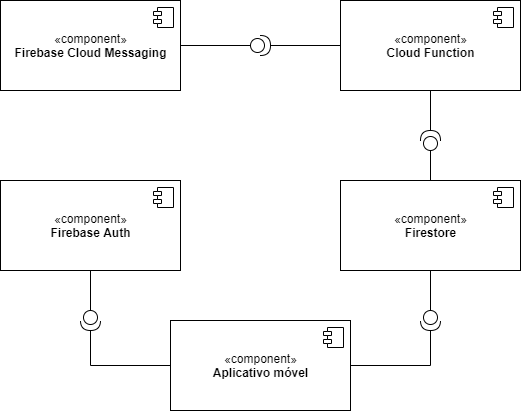
\includegraphics[scale=0.65]{diagrama-de-componentes.png}
  \caption{Diagrama de componentes.}
  \label{fig:diagramacomponentes}
\end{figure}

Cada um dos componentes do diagrama possui uma responsabilidade bem definida. O aplicativo móvel representa a interface do usuário e algumas regras de negócio que foram implementadas nas camadas interiores da \textit{Clean Architecture}.

O \textit{Firebase Auth} é o serviço responsável pela autenticação dos usuários, que nesse caso é utilizada apenas a autenticação anônima, como foi explicado nos capítulos anteriores.

O \textit{Firestore} representa o BD do sistema, que armazenará as localizações visitadas por cada usuário e as que forem classificadas como infectadas.

A \textit{Cloud Function} representa os \textit{scripts} que fazem a análise do rastreamento de contatos e possuem a responsabilidade de ativar o sistema de notificações se algum encontro entre usuários ocorrer.

O \textit{Firebase Cloud Messaging} é o serviço de envio de notificações.

Note que as conexões do diagrama mostram quais são os componentes que acessam as funcionalidades dos outros. Por exemplo, o aplicativo móvel não faz o envio de nenhuma notificação, a responsabilidade dessa tarefa são dos \textit{scripts} das \textit{Cloud Functions}.

\subsection{Modelagem das funcionalidades do sistema}
% Modelagem geral: casos de uso
% Modelagem de cada caso de uso: atividade e sequência
Cada funcionalidade do sistema foi herdada do levantamento de requisitos. Por conta disso, a partir do levantamento da Seção \ref{sec:requisitos}, foi criada a modelagem do diagrama de casos de uso, representado pela \Figura{fig:usecasesdiagram}. É importante ressaltar que este diagrama reflete a listagem de requisitos funcionais da Tabela \ref{tab:tabelaf}.

\begin{figure}[!htb]
  \centering
  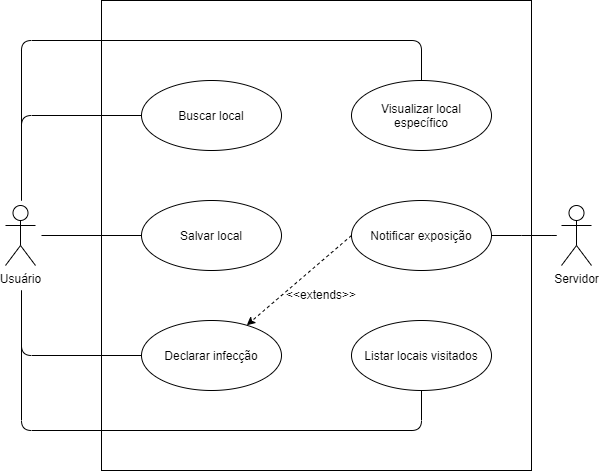
\includegraphics[scale=0.6]{Diagrama de casos de uso.png}
  \caption{Diagrama de casos de uso.}
  \label{fig:usecasesdiagram}
\end{figure}

Como cada caso de uso da \Figura{fig:usecasesdiagram} é uma funcionalidade, os diagramas de atividades e sequência foram modelados para cada um deles. Começando pelo "Buscar local", temos os respectivos diagrama de atividades na \Figura{fig:atividadebuscar} e o de sequência na \Figura{fig:sequenciabuscar}.

\begin{figure}[!htb]
  \centering
  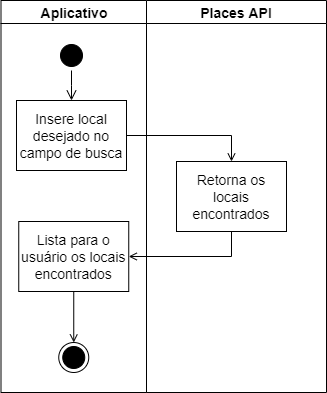
\includegraphics[scale=0.6]{Diagrama de atividades - Buscar.png}
  \caption{Diagrama de atividades da funcionalidade buscar local.}
  \label{fig:atividadebuscar}
\end{figure}

No diagrama de atividades da \Figura{fig:atividadebuscar} o usuário fará consultas em uma das APIs do \textit{Google}, chamada \textit{Places API}. Ela retornará qualquer localização no mundo que corresponda ao texto inserido pelo usuário.

\begin{figure}[!htb]
  \centering
  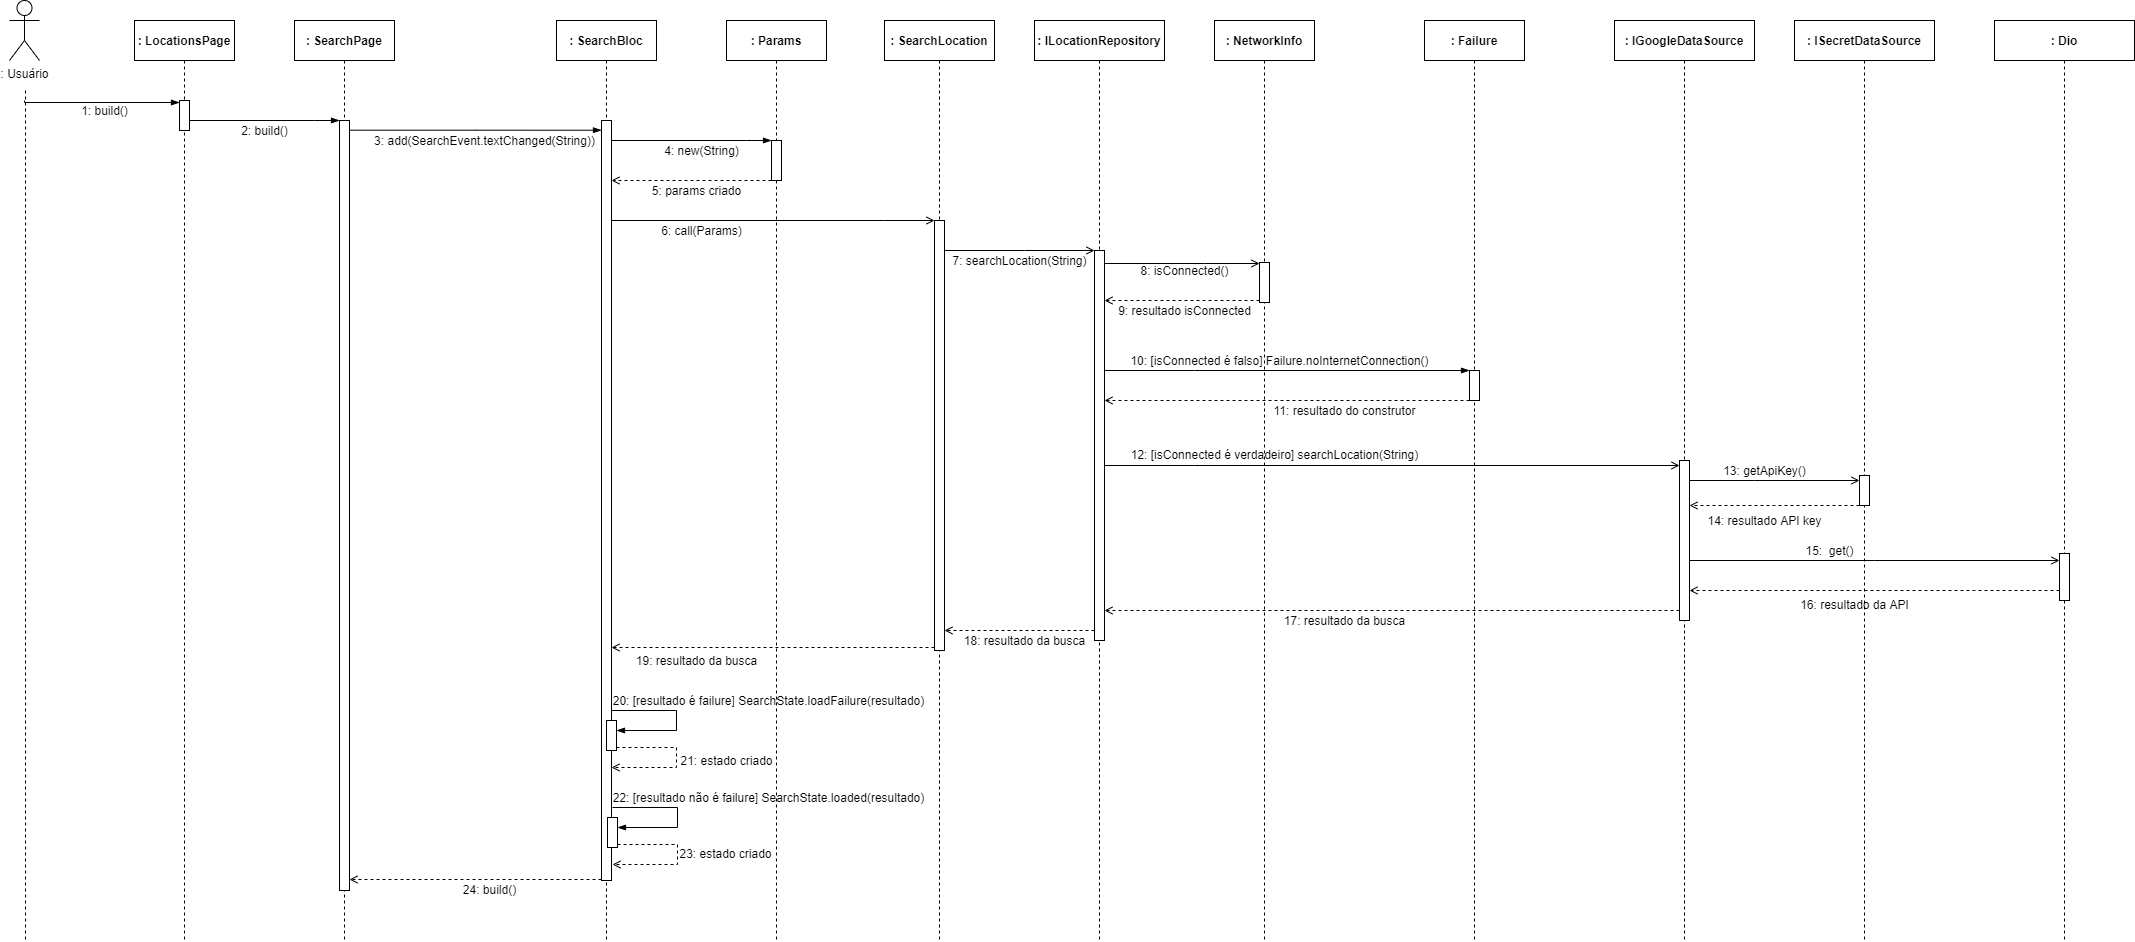
\includegraphics[scale=0.21]{Diagrama de sequencia - Buscar local.png}
  \caption{Diagrama de sequência da funcionalidade buscar local.}
  \label{fig:sequenciabuscar}
\end{figure}

Para a funcionalidade "Salvar local", a \Figura{fig:atividadesalvar} representa o diagrama de atividades, e o de sequência na \Figura{fig:sequenciasalvar}.

\begin{figure}[!htb]
  \centering
  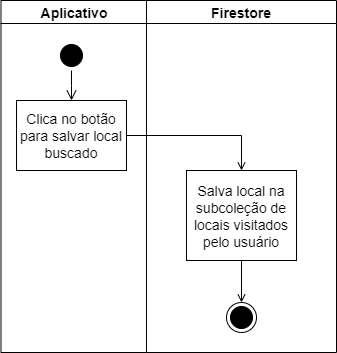
\includegraphics[scale=0.65]{Diagrama de atividades - Salvar.png}
  \caption{Diagrama de atividades da funcionalidade salvar local.}
  \label{fig:atividadesalvar}
\end{figure}

\begin{figure}[!htb]
  \centering
  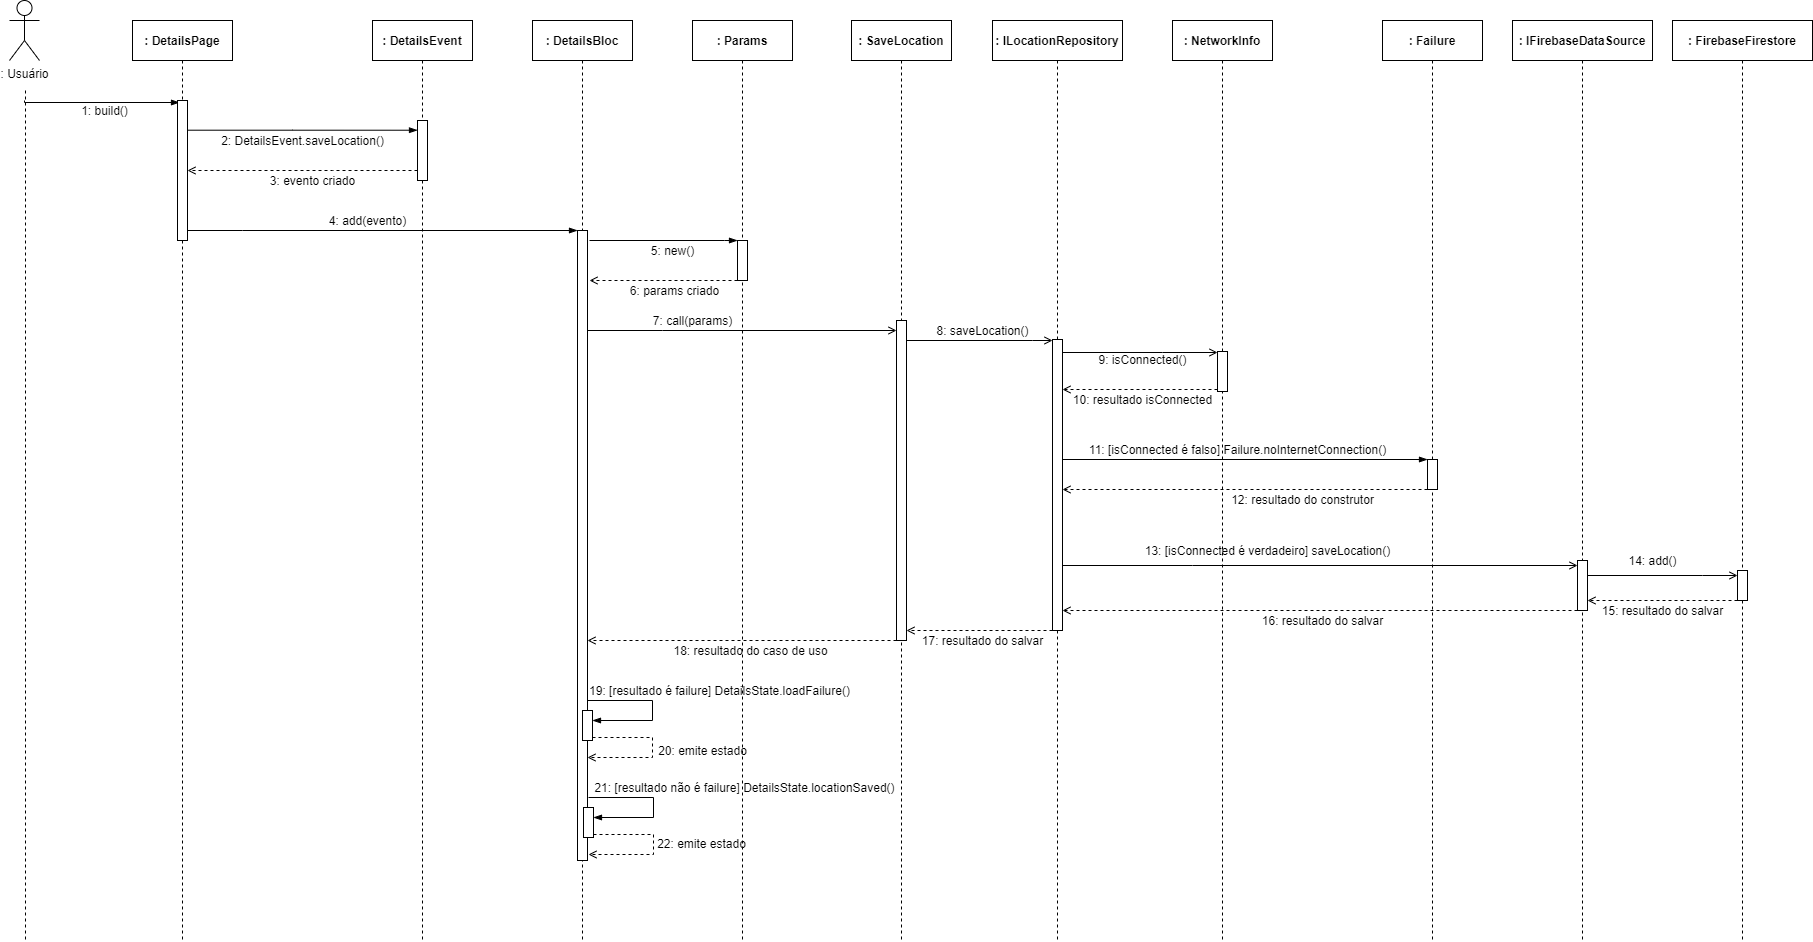
\includegraphics[scale=0.25]{Diagrama de sequencia - Salvar local.png}
  \caption{Diagrama de sequência da funcionalidade salvar local.}
  \label{fig:sequenciasalvar}
\end{figure}



A funcionalidade "Declarar infecção" está representada pelo diagrama de atividades da \Figura{fig:atividadedeclarar} e pelo de sequência da \Figura{fig:sequenciadeclarar}

\begin{figure}[!htb]
  \centering
  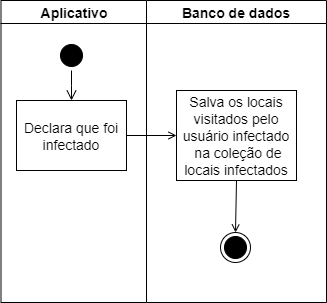
\includegraphics[scale=0.6]{Diagrama de atividades - Declarar.png}
  \caption{Diagrama de atividades da funcionalidade declarar infecção.}
  \label{fig:atividadedeclarar}
\end{figure}

\begin{figure}[!htb]
  \centering
  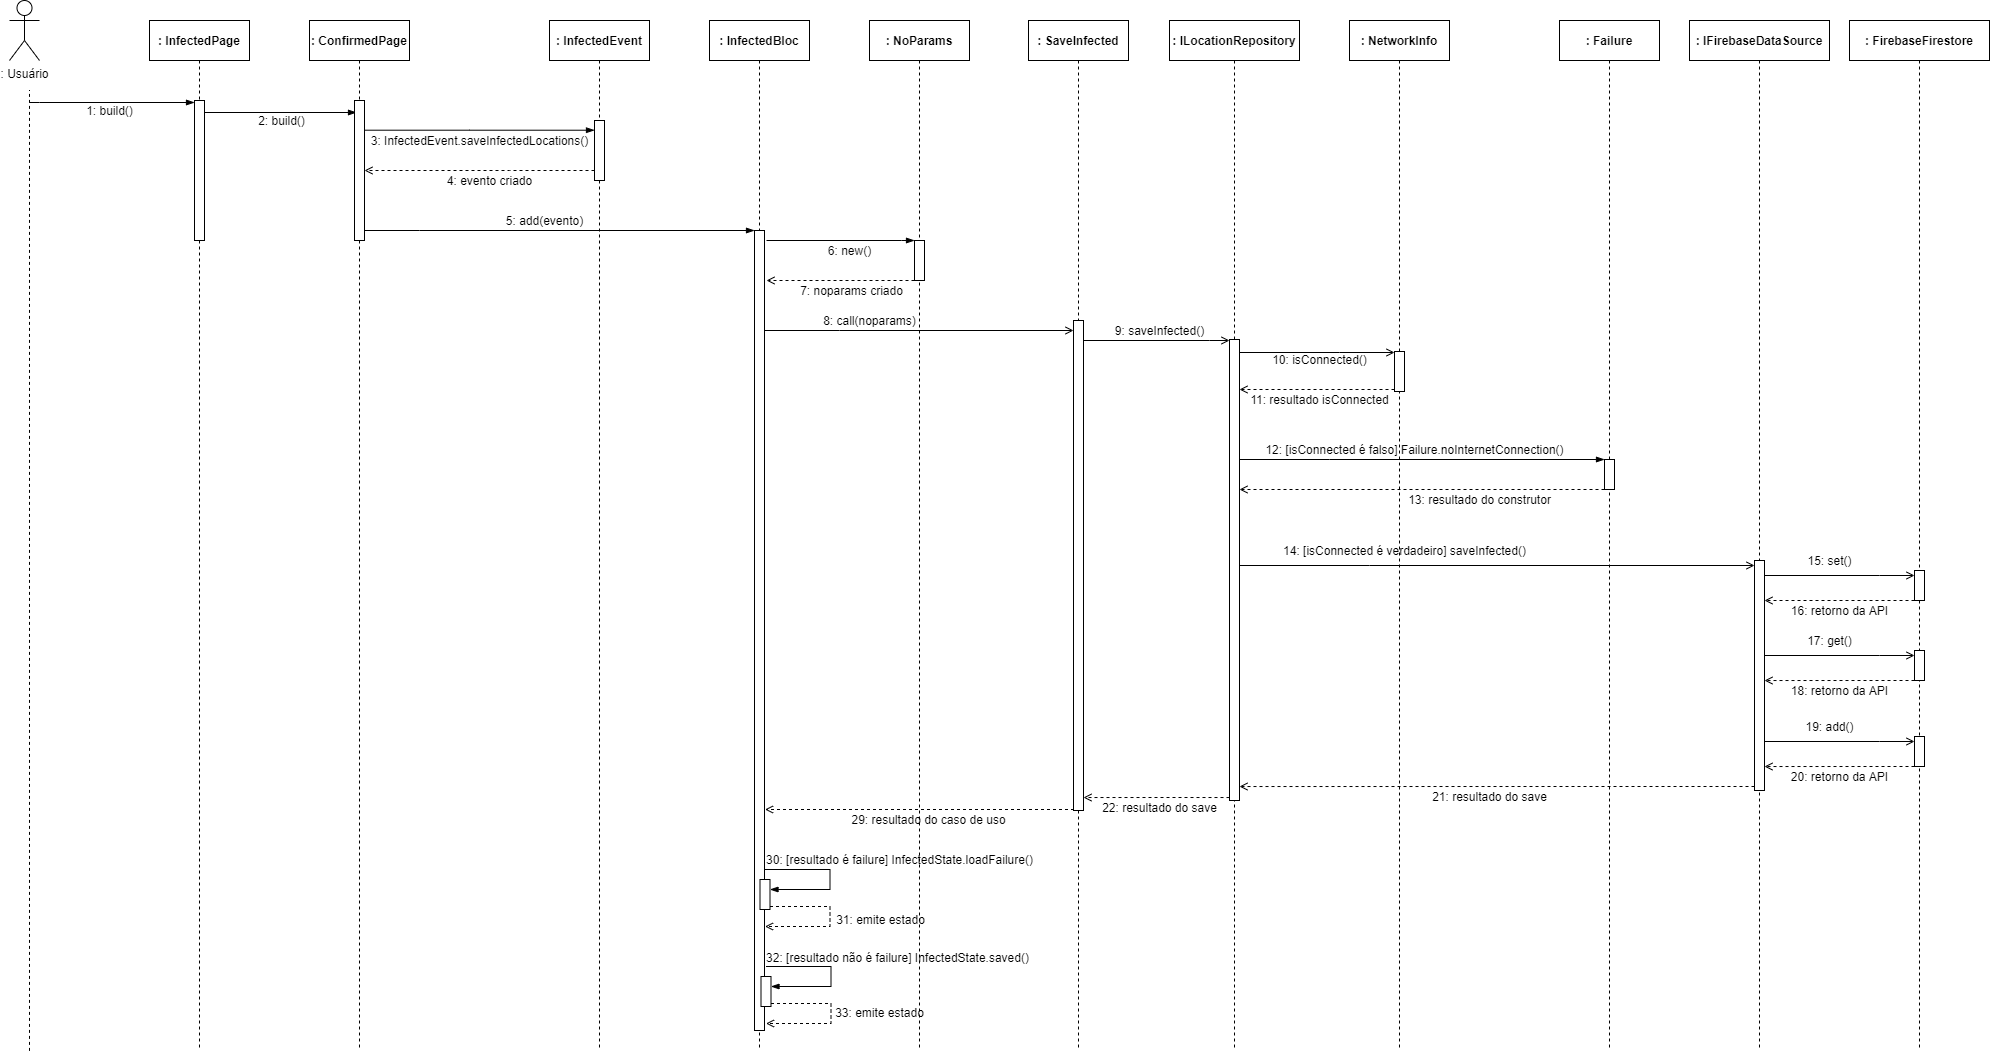
\includegraphics[scale=0.225]{Diagrama de sequencia - Declarar infeccao.png}
  \caption{Diagrama de sequência da funcionalidade declarar infecção.}
  \label{fig:sequenciadeclarar}
\end{figure}

Para a modelagem da funcionalidade "Visualizar local específico" temos a \Figura{fig:atividadevisualizar} para o diagrama de atividades e a \Figura{fig:sequenciavisualizar} para o de sequência.

\begin{figure}[!htb]
  \centering
  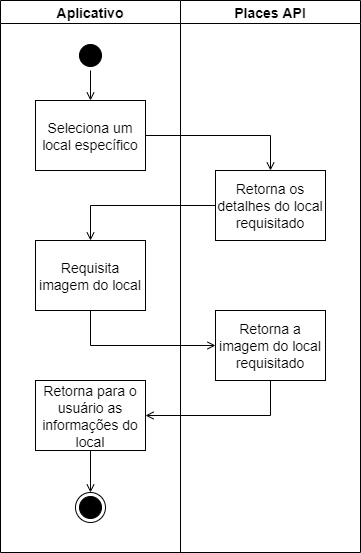
\includegraphics[scale=0.55]{Diagrama de atividades - Visualizar.png}
  \caption{Diagrama de atividades da funcionalidade visualizar local.}
  \label{fig:atividadevisualizar}
\end{figure}

\begin{figure}[!htb]
  \centering
  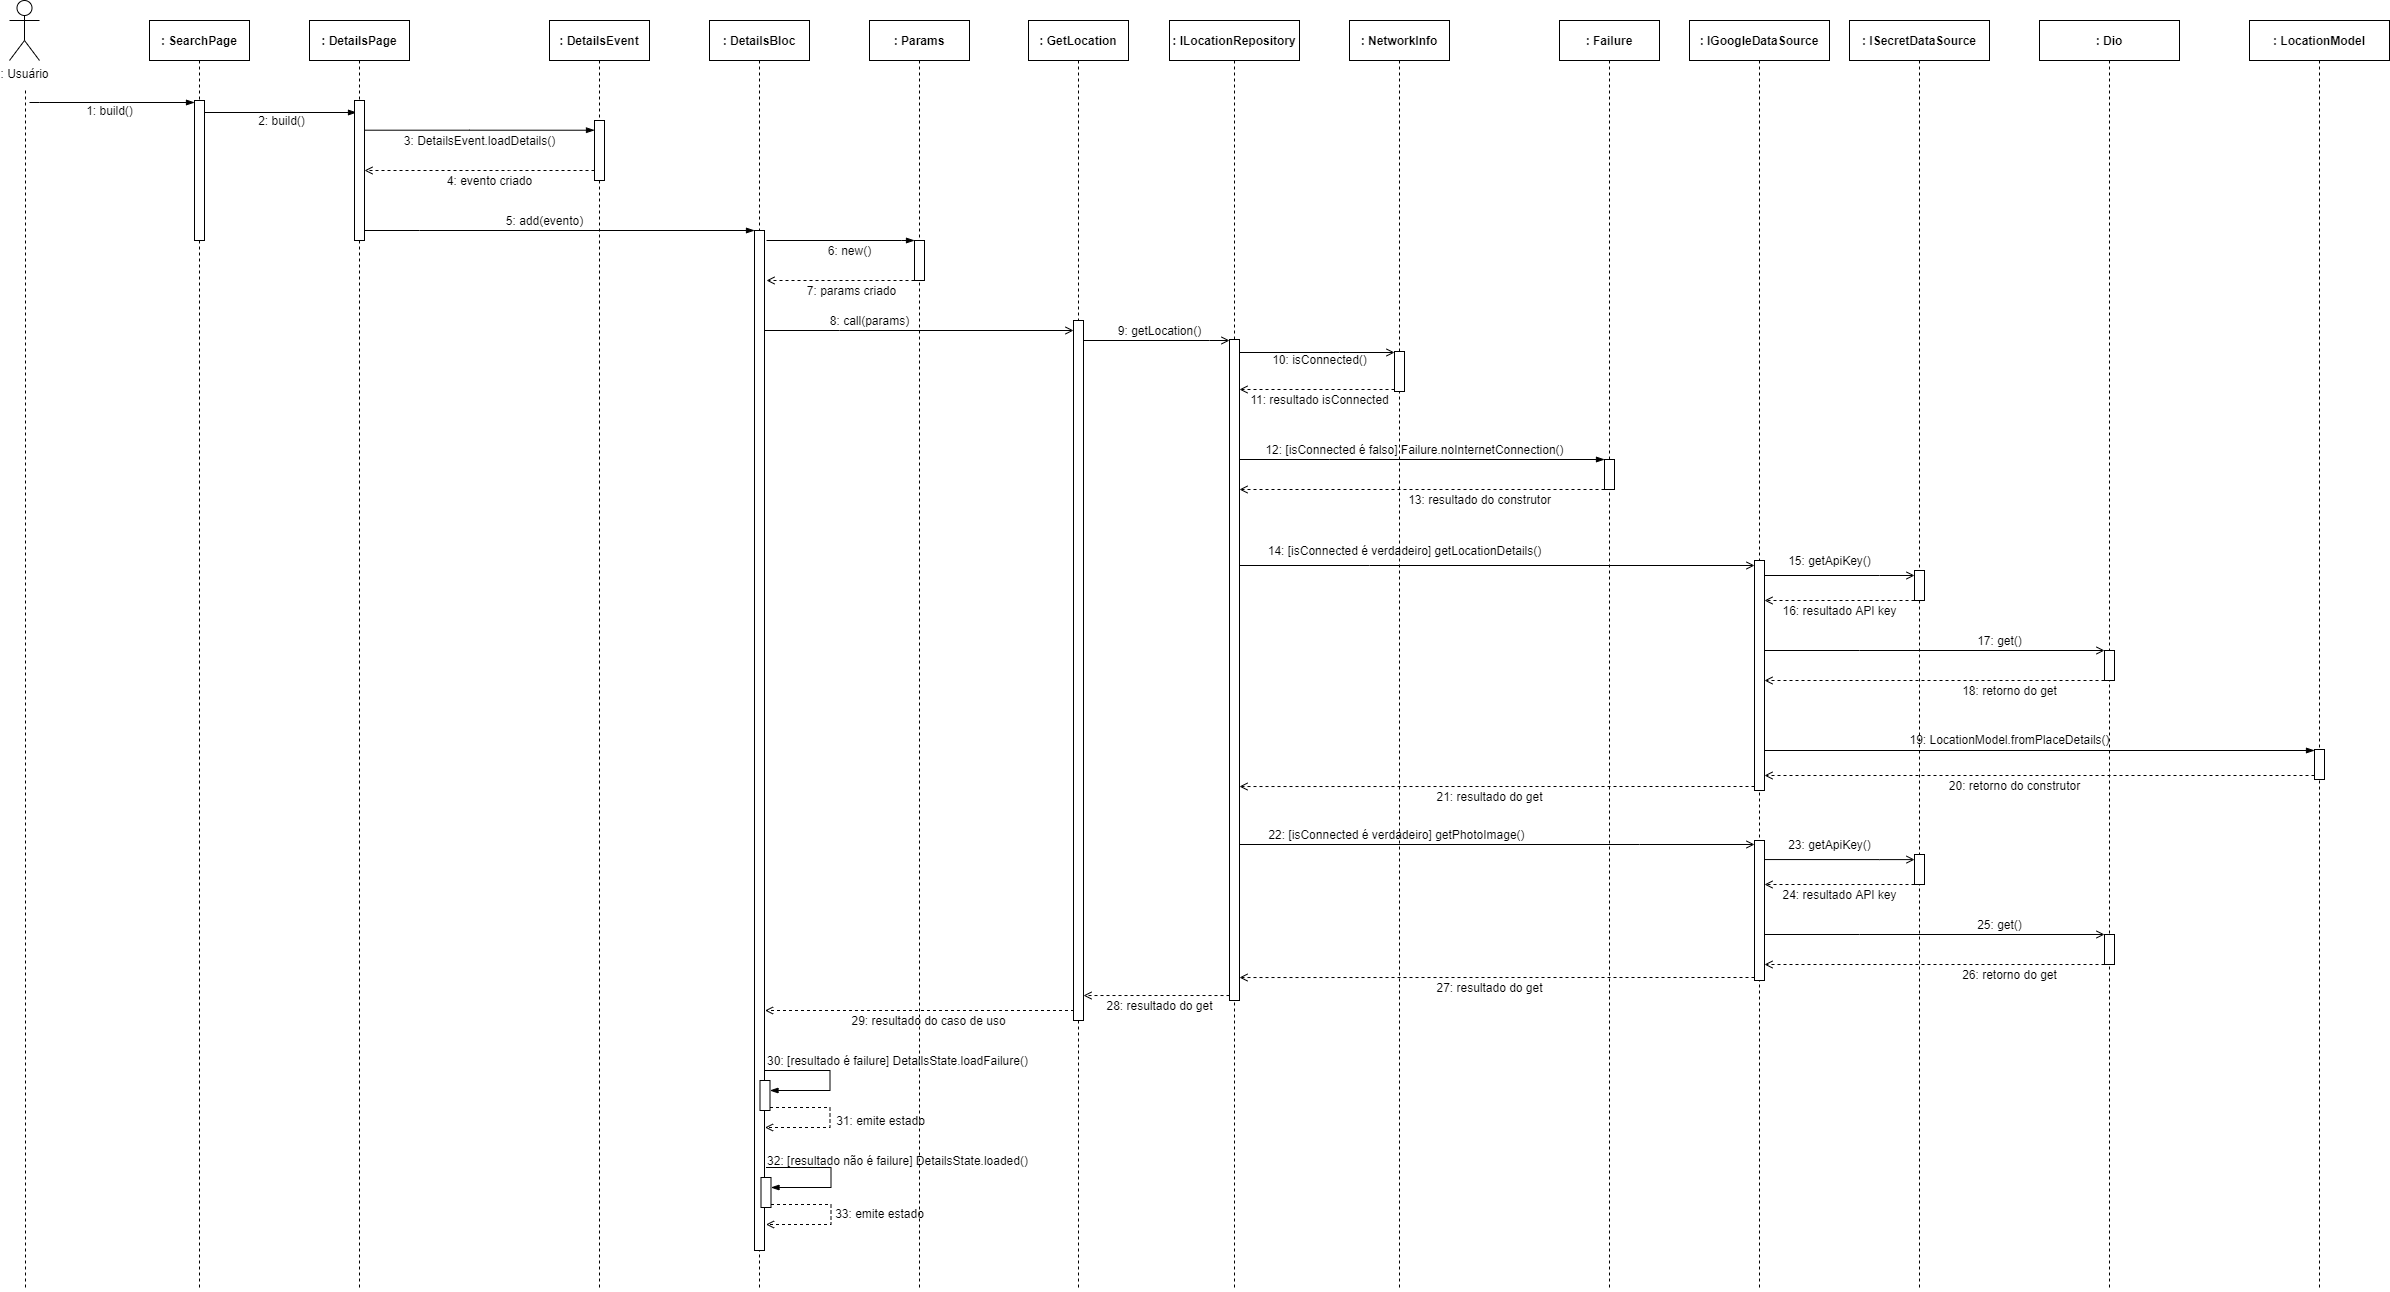
\includegraphics[scale=0.18]{Diagrama de sequencia - Visualizar local.png}
  \caption{Diagrama de sequência da funcionalidade visualizar local.}
  \label{fig:sequenciavisualizar}
\end{figure}

A funcionalidade "Notificar exposição" não possui um diagrama de sequência. Como essa funcionalidade vai ser atendida através do desenvolvimento de \textit{Cloud Functions}, a implementação não utiliza orientação a objetos, será um \textit{script} de análise de encontro entre usuários e não seria bem representado por objetos no diagrama.

Por conta disso, apenas o diagrama de atividades foi modelado e está representado pela \Figura{fig:atividadenotificar}.

\begin{figure}[!htb]
  \centering
  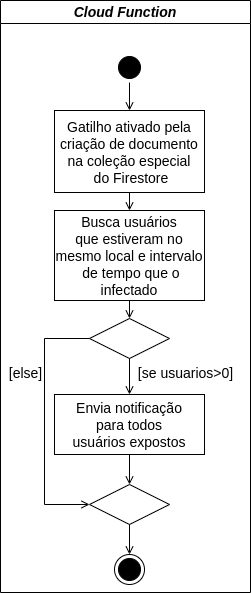
\includegraphics[scale=0.55]{Diagrama de atividades - Notificacao.png}
  \caption{Diagrama de atividades da funcionalidade notificar exposição.}
  \label{fig:atividadenotificar}
\end{figure}

Por último, a funcionalidade "Listar locais visitados" está representada pelo diagrama de atividades e de sequência da \Figura{fig:atividadelistar} e da \Figura{fig:sequencialistar}.

\begin{figure}[!htb]
  \centering
  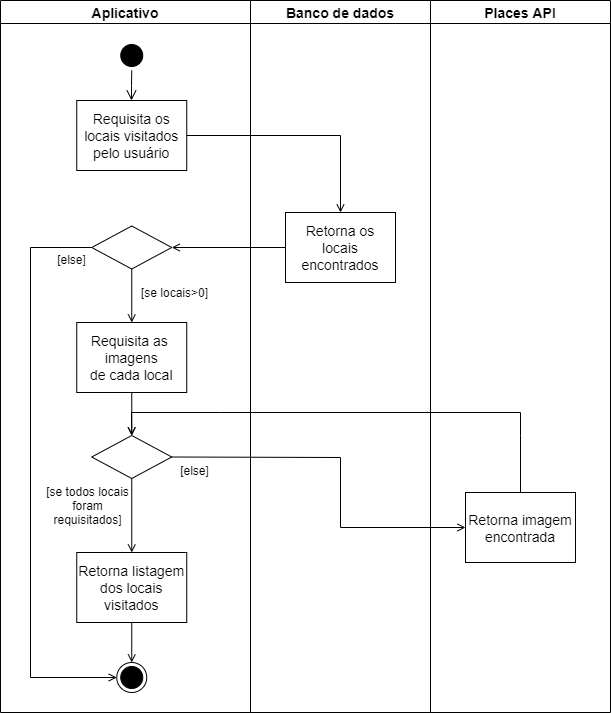
\includegraphics[scale=0.5]{Diagrama de atividades - Listar.png}
  \caption{Diagrama de atividades da funcionalidade listar locais.}
  \label{fig:atividadelistar}
\end{figure}

\begin{figure}[!htb]
  \centering
  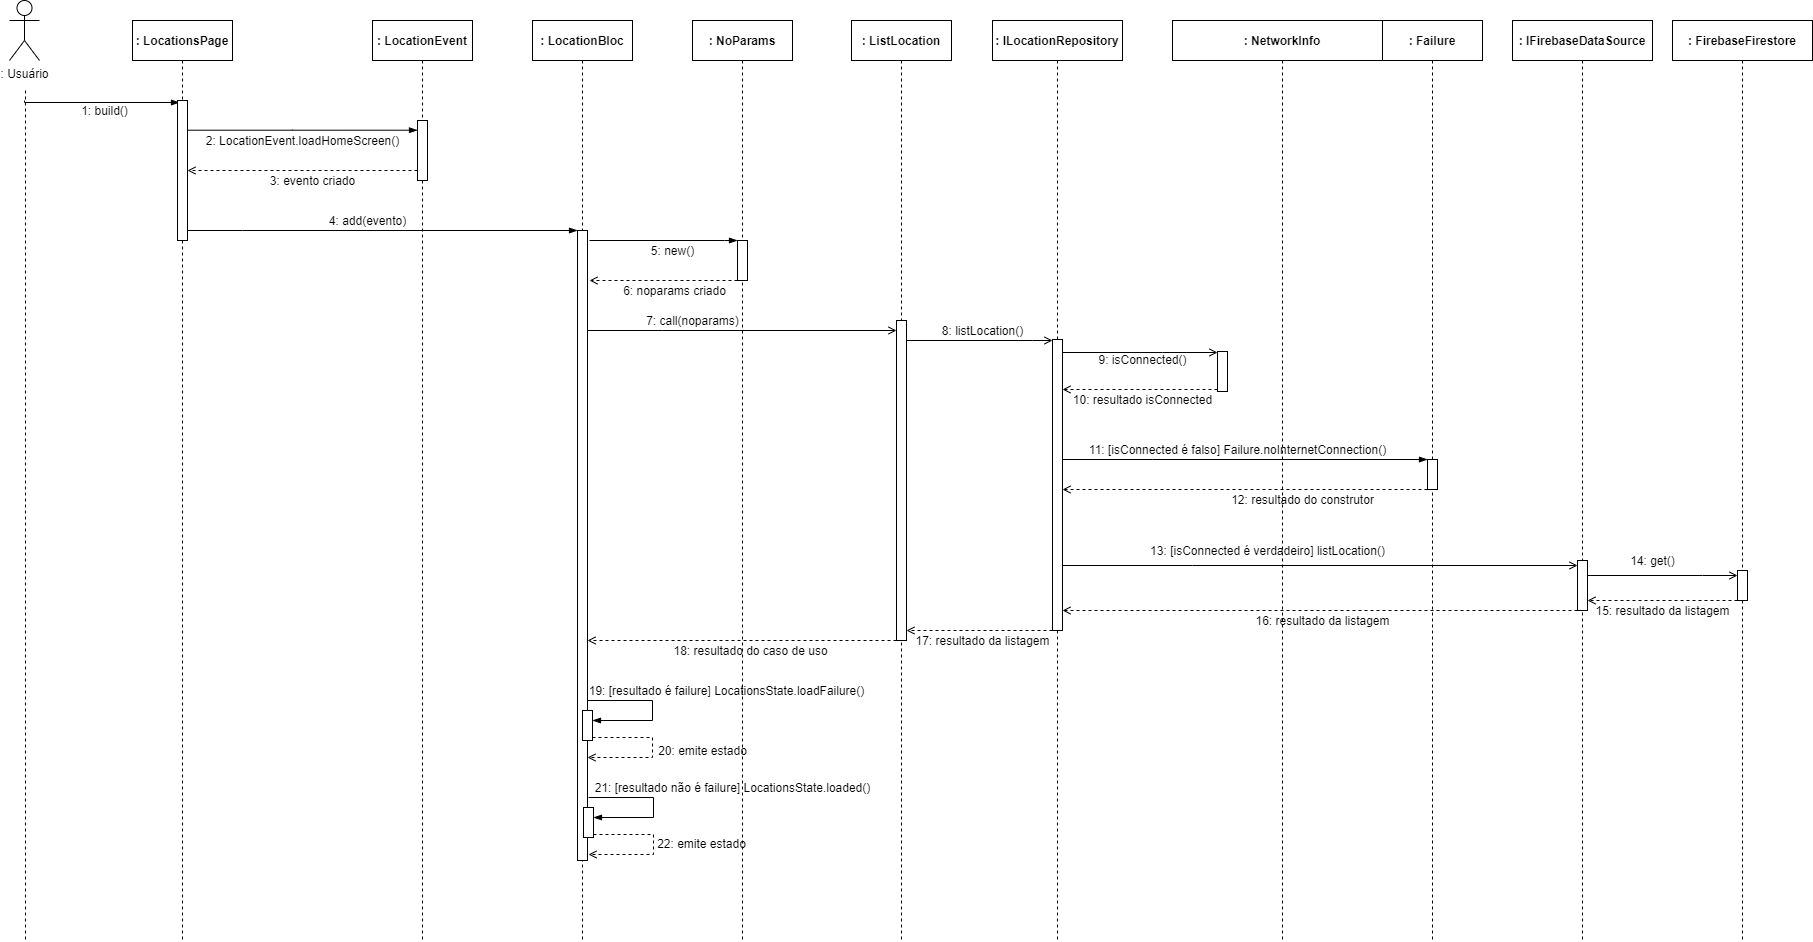
\includegraphics[scale=0.25]{Diagrama de sequencia - Listar locais.png}
  \caption{Diagrama de sequência da funcionalidade listar locais.}
  \label{fig:sequencialistar}
\end{figure}

\subsection{Modelagem da arquitetura do \textit{software}}
Como explicado na Seção \ref{sec:clean}, o aplicativo desenvolvido neste trabalho utiliza os princípios da arquitetura limpa. Por conta disso, a base da arquitetura do \textit{software} é a \Figura{fig:clean1}.

Antes de começar a diagramação, é importante entender a diferença entre dependência e fluxo de dados do aplicativo, porque essa diferença é crucial para que a modelagem não quebre nenhuma das regras da arquitetura limpa.

A dependência do código acontece no tempo de compilação, ou seja, só há dependência entre os componentes se houver uma referência direta para outro componente.

Por exemplo, imagine que em uma das classes da camada \textit{Application Business Rules} do aplicativo possua um caso de uso que em sua implementação exista uma chamada para um método de uma classe presente na camada \textit{Interface Adapters}. Nesse exemplo, o caso de uso possuiria dependência com a camada \textit{Interface Adapters}, e estaria ferindo a regra de dependência, já que essa é uma camada externa em relação à \textit{Application Business Rules}.

Já o fluxo de dados seria equivalente ao fluxo de chamadas dentro do código, que não acontece no tempo de compilação, e sim no de execução. Pode parecer contraditório, mas a dependência nem sempre reflete o fluxo de dados do código.

Utilizando o mesmo exemplo anterior, é possível fazer com que o caso de uso não dependa da camada \textit{Interface Adapters}, mas ainda consiga atingir o mesmo comportamento esperado. Para que isso aconteça, uma interface deve ser criada na camada \textit{Application Business Rules}, e ela conterá as assinaturas dos métodos que o caso de uso necessita. Na camada \textit{Interface Adapters}, uma classe implementará os métodos definidos na interface através do relacionamento de herança.

Dessa maneira, através do \textit{Dependency Inversion Principle}, explicado na subseção \ref{sec:D}, a dependência existirá da camada \textit{Interface Adapters} para a camada \textit{Application Business Rules} por conta da herança, mas no fluxo de chamadas em tempo de execução, será da \textit{Application Business Rules} para a camada \textit{Interface Adapters}.

Com a diferença entre dependência e fluxo de dados compreendida, toda modelagem da arquitetura do sistema deve fazer com que nenhuma camada interna dependa de uma mais externa à ela. Para isso, todas as fronteiras das camadas haverão interfaces para possibilitar a comunicação sem que a regra de dependência seja ferida.

Como o aplicativo fará chamadas para componentes de persistência de dados, utilizando APIs para busca de locais e um BD remoto para o armazenamento, essas chamadas serão realizadas utilizado o padrão de repositório. A partir disso, o fluxo dos dados entre os componentes do sistema serão nessa ordem:

\begin{enumerate}
  \item \textit{View} faz chamadas dos métodos da \textit{View Model};
  \item \textit{View Model} executa o caso de uso;
  \item Caso de uso combina os dados dos repositórios das entidades;
  \item Cada repositório retorna os dados dos \textit{Data Sources};
  \item Os dados voltam para a \textit{View} e são mostrados ao usuário;
\end{enumerate}

A partir dessa ordem, a adaptação da \Figura{fig:clean1} com o padrão de repositório e da diferença entre dependência e fluxo de dados é representada na \Figura{fig:cleanadapt}.

\begin{figure}[!htb]
  \centering
  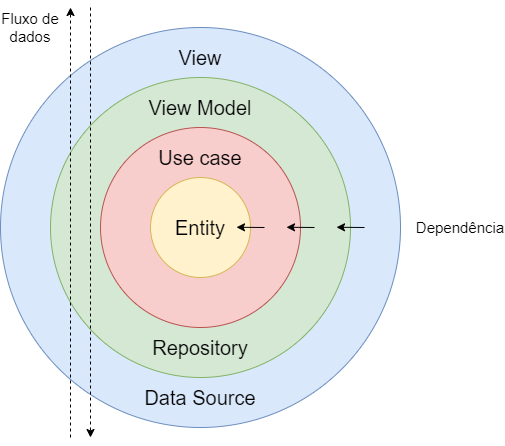
\includegraphics[scale=0.5]{clean-adapt.png}
  \caption{Diferença entre dependência e fluxo de dados.}
  \label{fig:cleanadapt}
\end{figure}

Note que as dependências estão sempre apontando para o interior. Levando em consideração a explicação de como as fronteiras das camadas são passadas através da inversão de dependências, o diagrama de pacotes da \Figura{fig:package} possui a modelagem mais abstrata e de maior alto nível da arquitetura do aplicativo. 

% imagem do diagrama de pacotes 
\begin{figure}[!htb]
  \centering
  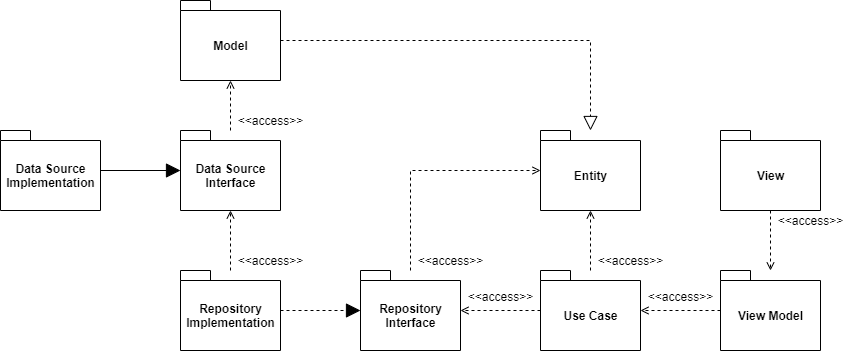
\includegraphics[scale=0.5]{Diagrama de pacotes.png}
  \caption{Diagrama de pacotes do aplicativo.}
  \label{fig:package}
\end{figure}

Para que a associação do diagrama da \Figura{fig:package} com as camadas e regras de dependência da \Figura{fig:cleanadapt} sejam melhor visualizadas, a \Figura{fig:package2} representa as camadas da arquitetura limpa com as mesmas colorações por cima do diagrama de pacotes.

\begin{figure}[!htb]
  \centering
  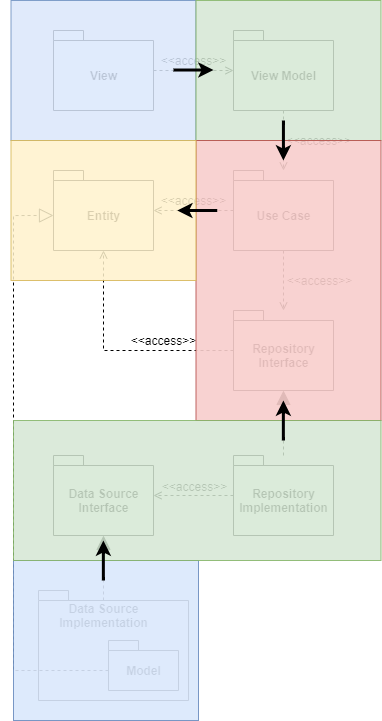
\includegraphics[scale=0.43]{package-adapt.png}
  \caption{Diagrama de pacotes com as colorações das camadas da arquitetura limpa.}
  \label{fig:package2}
\end{figure}

Com todos diagramas mostrados anteriormente modelados, o diagrama de classes foi feito com base nos outros e pode ser visualizado na \Figura{fig:diagramadeclasses}. Como alguns diagramas ficaram grandes, a visualização deles fica impossibilitada nas páginas deste trabalho, por isso, visualize a pasta figuras\footnote{Disponível em: <https://github.com/Feggah/tcc/tree/main/docs/figuras>. Acesso em: 21 out. 2021.} no repositório do \textit{GitHub} para uma visão mais detalhada.

\begin{figure}[!htb]
  \centering
  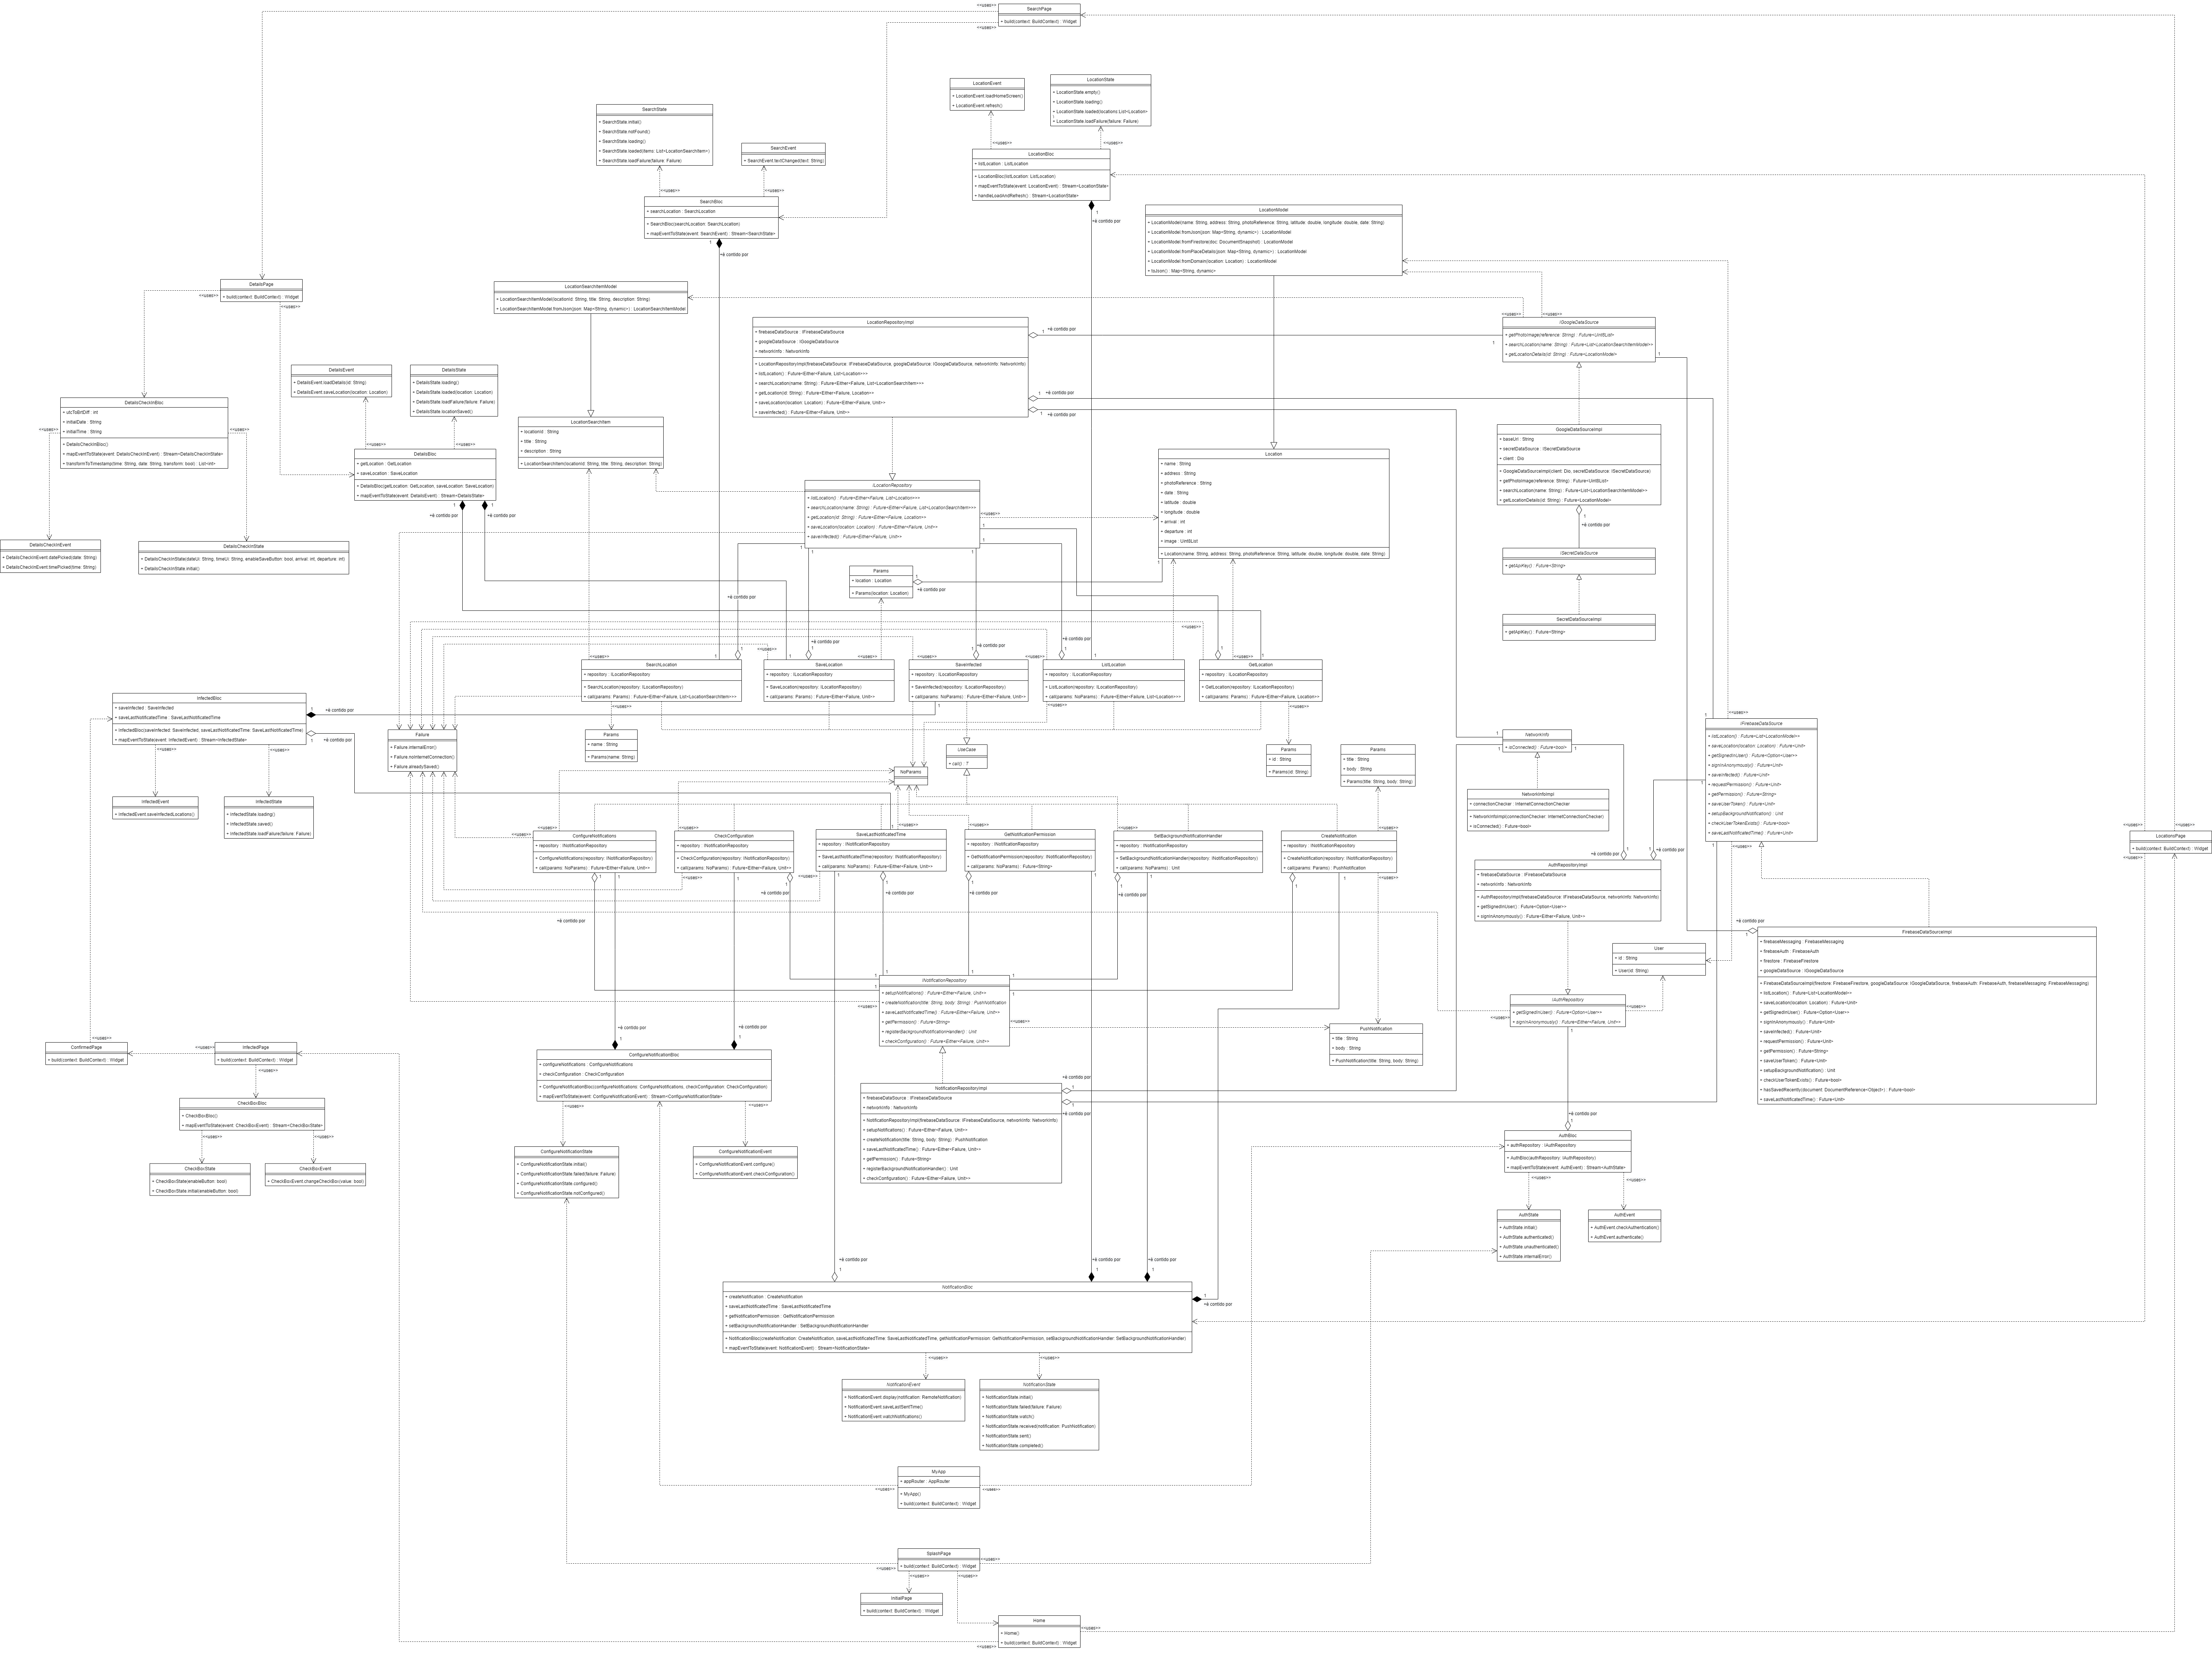
\includegraphics[scale=0.075]{Diagrama de classes.png}
  \caption{Diagrama de classes do aplicativo.}
  \label{fig:diagramadeclasses}
\end{figure}

\subsection{Modelagem de dados}\label{sec:modelagemdedados}
O sistema de rastreamento de dados necessita apenas de algumas informações persistidas sobre os usuários para que a análise de encontro entre eles seja efetuada com sucesso. 

Para cada usuário deverá ser armazenado os locais visitados e um identificador aleatório que possibilita o envio de notificações ao seu dispositivo móvel. Para isso, será utilizado uma coleção no \textit{Firestore} chamada \textit{users}. Nela serão armazenados múltiplos documentos, em que cada um representa um usuário. Em cada documento haverá o \textit{token} e a subcoleção dos locais visitados.

Além disso, dois campos opcionais também serão necessários. Um deles garantirá que o usuário não seja notificado múltiplas vezes em um curto período de tempo, o outro garantirá que ele não consiga se declarar como infectado múltiplas vezes dentro do período de 14 dias. O nome desses dois campos são respectivamente chamados de \textit{lastNotified} e \textit{lastSaved}.

Os documentos que representam os locais visitados serão compostos por alguns valores de retorno da API do \textit{Google}, que são os campos endereço, latitude, longitude, nome e o ID da foto. Para armazenar o horário que o usuário esteve no local, serão utilizados campos no formato \textit{timestamp} do horário de chegada e de saída que forem preenchidos pelo usuário na interface do aplicativo.

Os locais considerados como infectados serão armazenados em outra coleção com o objetivo de diminuição de profundidade da estrutura do BD, resultando em menos requisições de leitura. A consequência disso é que o tempo de processamento do algoritmo de análise de rastreamento e os custos da nuvem diminuirão, porque será necessário apenas uma requisição de leitura para obter todos os locais infectados e o valor cobrado é diretamente relacionado com o número de requisições efetuadas.

Essa coleção tem o nome \textit{infected} e cada um de seus documentos representam um local, contendo o horário, latitude e longitude do local classificado como infectado.

Como resultado desse racional apresentado acima, a modelagem da \Figura{fig:modelagemfirestore} representa a estrutura e todos atributos obrigatórios e opcionais de cada documento.

\begin{figure}[!htb]
  \centering
  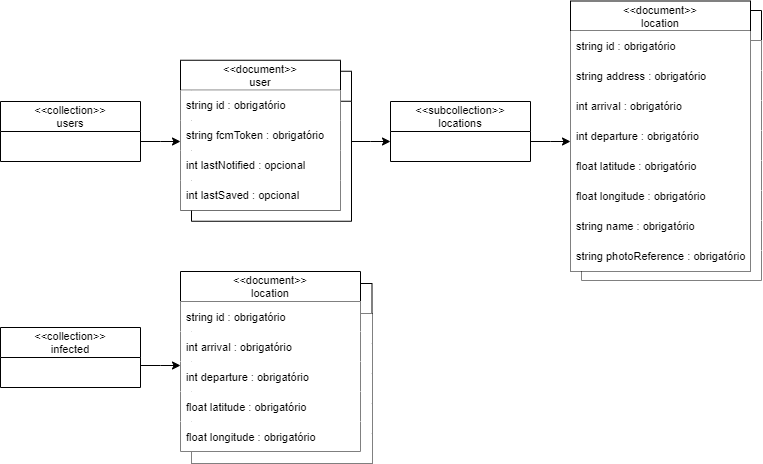
\includegraphics[scale=0.59]{Modelagem banco de dados.png}
  \caption{Modelagem do banco de dados não relacional.}
  \label{fig:modelagemfirestore}
\end{figure}

\section{Interfaces de usuário do aplicativo}\label{sec:uiux}
O \textit{design} das interfaces do aplicativo foi criado utilizando o \textit{Figma}, que é um editor online gratuito de gráficos vetoriais com ênfase na prototipagem de interfaces gráficas. Todos protótipos de tela construídos podem ser visualizados na página do projeto\footnote{Disponível em: <https://www.figma.com/file/x11PMoHwniQ0e1Jb6T6LRk/TCC>. Acesso em: 23 out. 2021.} dentro da ferramenta. 

As principais telas do aplicativo são as que estão diretamente associadas à uma das funcionalidades da Tabela \ref{tab:tabelaf} e representadas pelo diagrama de casos de uso da \Figura{fig:usecasesdiagram}, que são as telas de listagem, busca e visualização de locais e a de declaração de caso de infecção. Os protótipos das quatro telas podem ser visualizados na \Figura{fig:principaistelas}.

\begin{figure}[!htb]
  \centering
  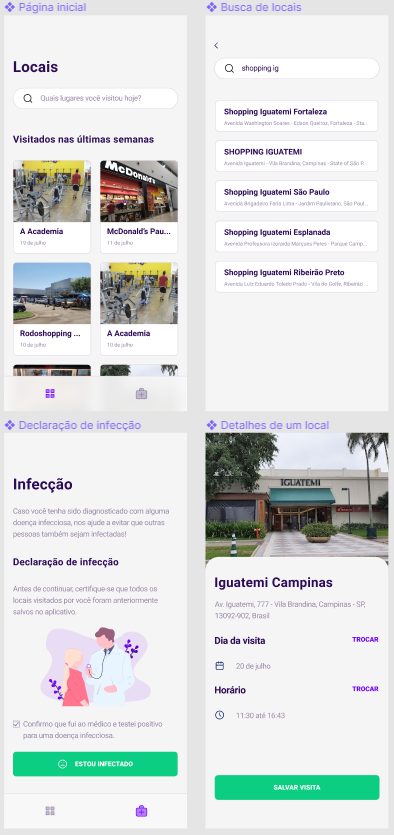
\includegraphics[scale=0.8]{interface-principais-telas.png}
  \caption{Protótipo das principais telas do aplicativo móvel.}
  \label{fig:principaistelas}
\end{figure}

Além das quatro telas principais, existem algumas variações das mesmas em casos de erro, falta de conexão com a \textit{Internet} e páginas de \textit{feedback} para alguma ação do usuário. Por exemplo, quando o usuário se auto declara como infectado, ele visualizará uma página de confirmação informando que o processamento foi concluído com sucesso.

\section{Implementação}\label{sec:implementacao}

As tarefas necessárias para conclusão do projeto foram criadas no formato de \textit{issues} no repositório do \textit{GitHub}. Cada issue foi classificada entre \textit{feature}, \textit{release}, \textit{diagram} e \textit{documentation} através de rótulos adicionados à elas.

O rótulo de \textit{release} significa que aquela \textit{issue} será concluída no momento que uma nova versão do sistema seja lançada. Isso também significa que uma \textit{release} contém várias \textit{issues} do tipo \textit{feature} que devem ser concluídas primeiramente.

Um exemplo de \textit{release} foi o lançamento do \Sigla{\textit{Minimum viable product}}{MVP}, que continha como pré-requisito a conclusão de todas as \textit{issues} que representavam as funcionalidades levantadas na Seção \ref{sec:requisitos}. A \Figura{fig:issuemvp} é um \textit{printscreen} que mostra como foi estruturada as \textit{issues} do repositório.

\begin{figure}[!htb]
  \centering
  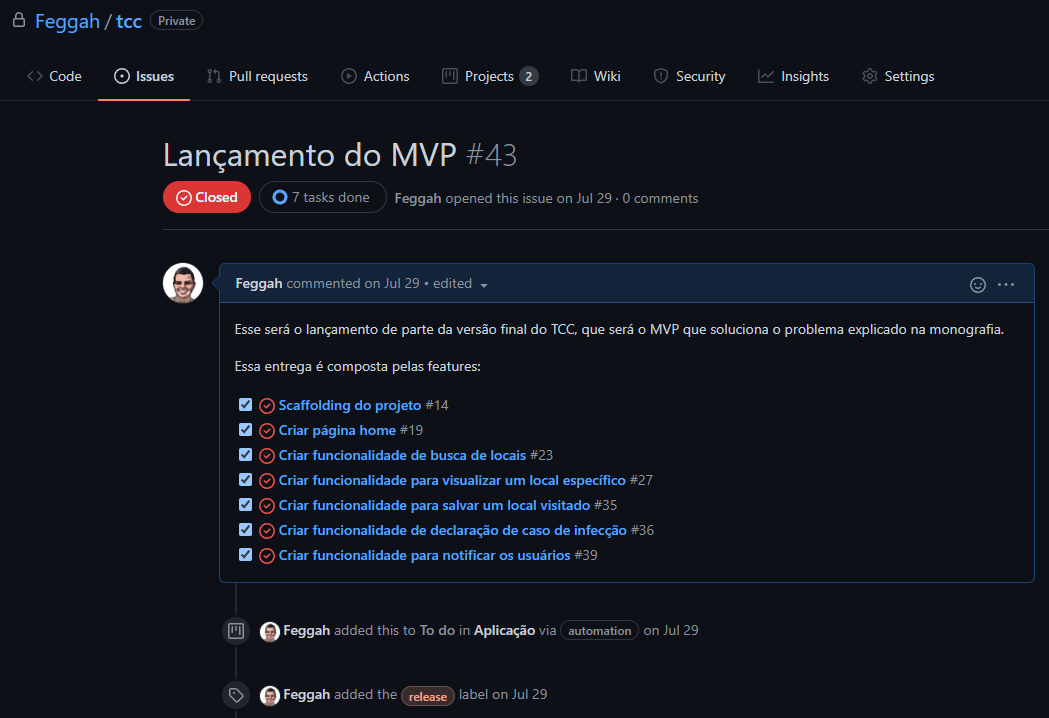
\includegraphics[scale=0.57]{mvp-issue.png}
  \caption{\textit{Printscreen} da \textit{issue} de lançamento do MVP.}
  \label{fig:issuemvp}
\end{figure}

Todas as \textit{issues} seguem esse mesmo modelo: possuem um título, descrição do que deve ser feito e um rótulo classificando qual o seu tipo.

O rótulo \textit{feature} representa uma funcionalidade a ser implementada no sistema. Essa funcionalidade não deve necessariamente representar uma relação um para um com as funcionalidades levantadas na Seção \ref{sec:requisitos}, ou seja, elas podem ser quebradas em entregas menores.

O rótulo \textit{documentation} está relacionado a tarefas de desenvolvimento do texto da monografia. Por exemplo, uma \textit{issue} que representa o desenvolvimento de um dos capítulos deste trabalho.

A última classificação, o rótulo \textit{diagram}, representa tarefas que estavam relacionadas a modelagem dos diagramas criados para este trabalho. No caso desse rótulo, foi utilizado uma \textit{issue} para cada tipo de diagrama, por exemplo, a \textit{issue} sobre o diagrama de atividades representava a modelagem dos seis diagramas criados. 

Para que a visualização e progresso das \textit{issues} fosse melhor visualizado, foi utilizado um quadro \textit{Kanban} oferecido nativamente pelo \textit{GitHub}, que são chamados de projetos. Foram criados dois projetos, um representando a implementação de todo o sistema e o outro o desenvolvimento da monografia e assuntos relacionados.

Os dois quadros \textit{Kanbans} foram divididos em três colunas: \textit{To do}, \textit{in progress} e \textit{done}. As \textit{issues} que estavam dentro de cada quadro eram movidas conforme o seu estado mudava em relação a coluna que ela estava inserida. Por exemplo, a \Figura{fig:kanbanmono} representa o estado do quadro da monografia durante o desenvolvimento desta seção.

\begin{figure}[!htb]
  \centering
  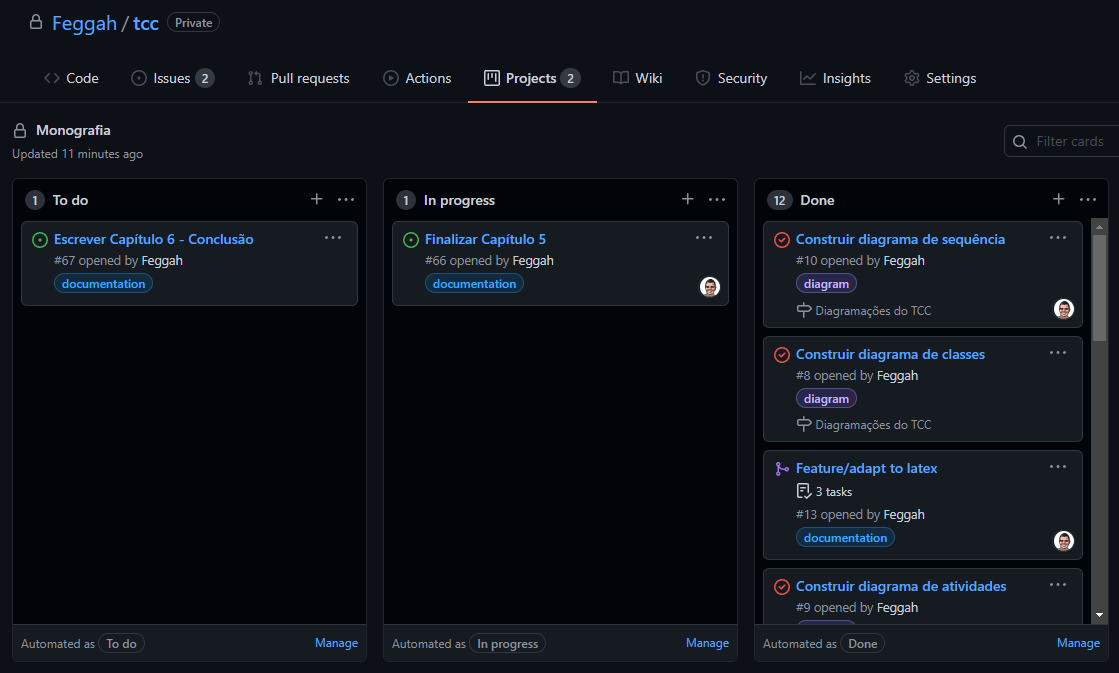
\includegraphics[scale=0.53]{kanban-github.png}
  \caption{\textit{Printscreen} do quadro \textit{Kanban} da monografia.}
  \label{fig:kanbanmono}
\end{figure}

Como explicado na Seção \ref{sec:Git}, o fluxo de trabalho escolhido para o processo de desenvolvimento do sistema foi o \textit{GitFlow}. Por conta disso, o repositório possui duas ramificações de longa vida, a \textit{main} e a \textit{develop}.

Para exemplificar o fluxo completo do \textit{GitFlow} na prática, a \Figura{fig:cfpr} possui um exemplo de \textit{pull request} para a ramificação \textit{develop}.

\begin{figure}[!htb]
  \centering
  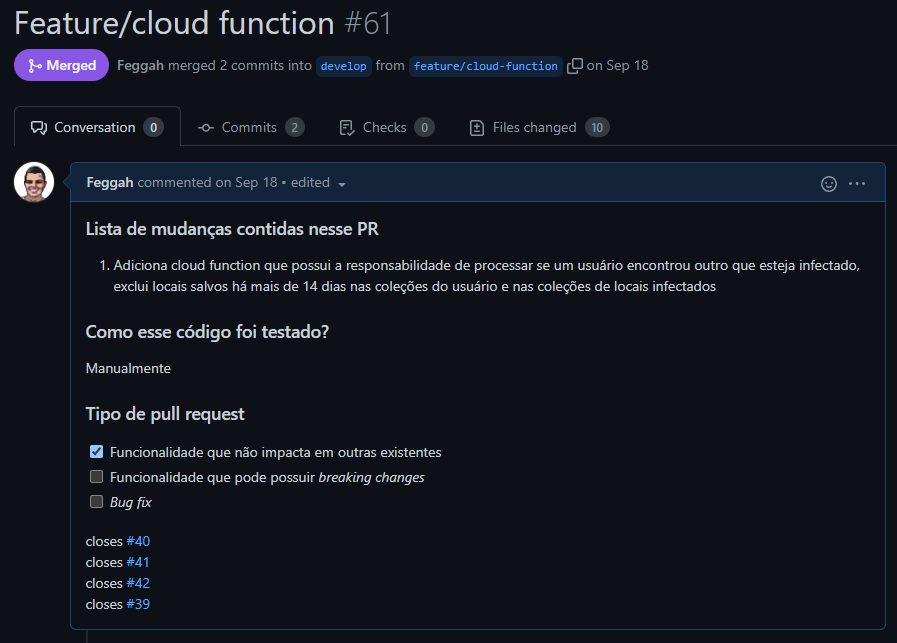
\includegraphics[scale=0.65]{pr-to-develop-example.png}
  \caption{\textit{Printscreen} de exemplo de um \textit{pull request} do repositório.}
  \label{fig:cfpr}
\end{figure}

Depois de algumas iterações de funcionalidades mescladas na ramificação \textit{develop}, a ramificação \textit{release} é criada a partir da \textit{develop} e são criados dois \textit{pull requests}, um para a \textit{main} e outro para a \textit{develop}. A \Figura{fig:releasemainpr} representa o \textit{pull request} para a main e a \Figura{fig:releasedeveloppr} para a \textit{develop}.

\begin{figure}[!htb]
  \centering
  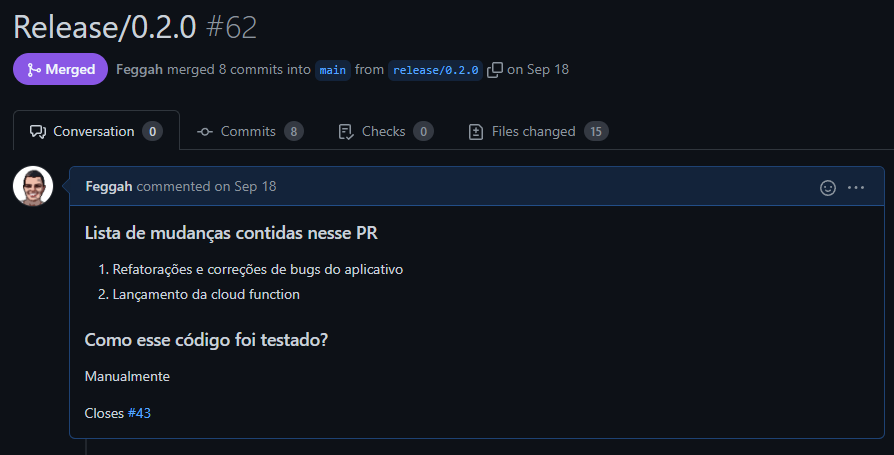
\includegraphics[scale=0.65]{pr-release-to-main.png}
  \caption{\textit{Printscreen} de exemplo de um \textit{pull request} da ramificação \textit{release} para \textit{main} do repositório.}
  \label{fig:releasemainpr}
\end{figure}

\begin{figure}[!htb]
  \centering
  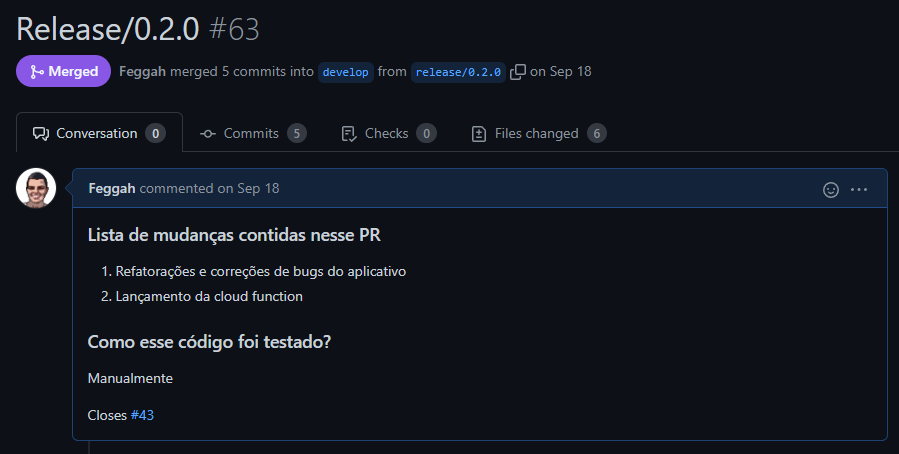
\includegraphics[scale=0.65]{pr-release-to-develop.png}
  \caption{\textit{Printscreen} de exemplo de um \textit{pull request} da ramificação \textit{release} para \textit{develop} do repositório.}
  \label{fig:releasedeveloppr}
\end{figure}

Com isso, a ramificação principal do repositório possui as novas funcionalidades desenvolvidas e uma nova versão está pronta para ser lançada. O lançamento de versão é feito adicionando uma \textit{tag}, que fixa um ponto histórico no repositório e representa uma versão da aplicação.

Com a nova \textit{tag} criada, um novo lançamento é feito através da funcionalidade de \textit{releases} do \textit{GitHub}. Uma \textit{release} contém título, descrição, a \textit{tag} que está associada à ela e arquivos que possam fazer parte desse lançamento. No caso do aplicativo, uma release contém o arquivo \Sigla{\textit{Android Package}}{APK} que pode ser baixado e instalado nos dispositivos. A \Figura{fig:currentreleases} representa os lançamentos feitos no repositório.

\begin{figure}[!htb]
  \centering
  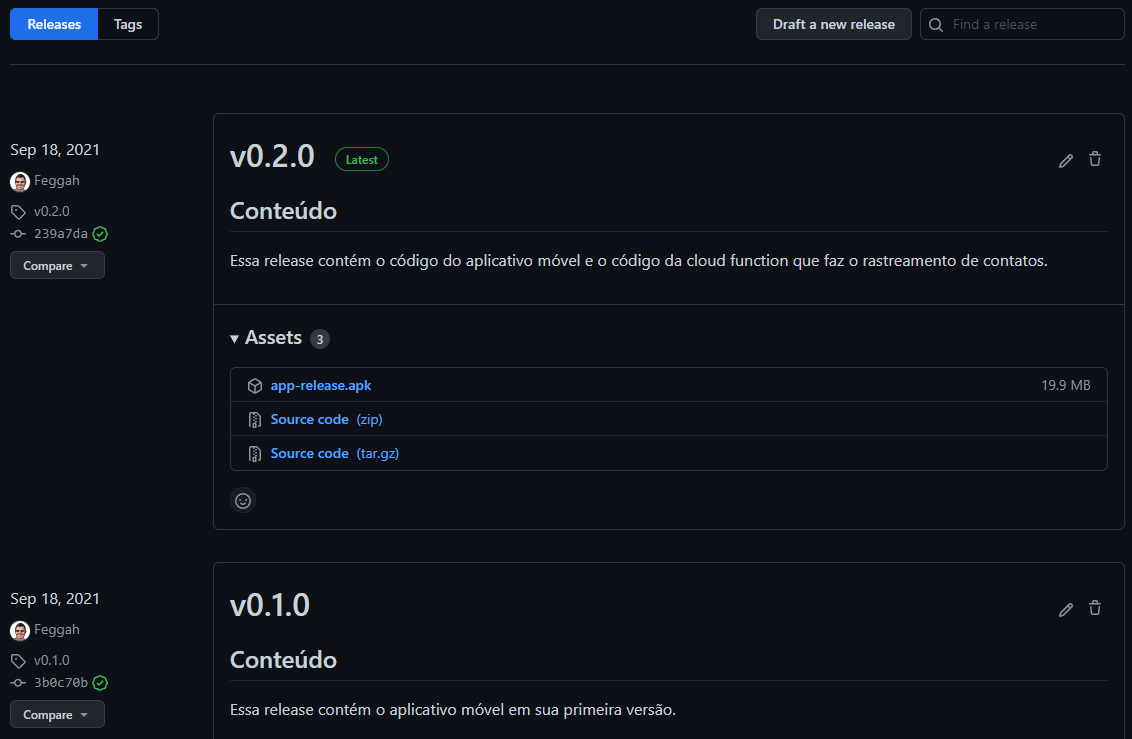
\includegraphics[scale=0.53]{repo-releases.png}
  \caption{\textit{Printscreen} das \textit{releases} do repositório.}
  \label{fig:currentreleases}
\end{figure}

Além do fluxo usual de incremento de funcionalidades, algumas correções pontuais podem ser feitas na versão que já está na ramificação principal através de ramificações denominadas de \textit{hotfix}. A \Figura{fig:hotfixpr} representa um exemplo desse tipo de modificação.

\begin{figure}[!htb]
  \centering
  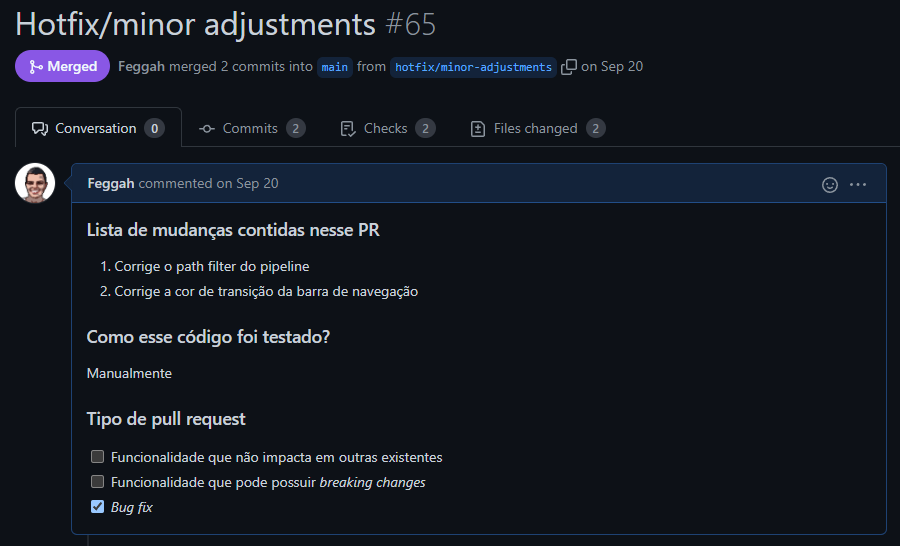
\includegraphics[scale=0.65]{pr-hotfix.png}
  \caption{\textit{Printscreen} de exemplo de um \textit{pull request} de \textit{hotfix}.}
  \label{fig:hotfixpr}
\end{figure}

Como o fluxo de trabalho escolhido utiliza o modelo de \textit{pull requests}, é importante que em cada um rode os testes automatizados, a fim de garantir que as novas modificações não estão quebrando o comportamento de funcionalidades antigas.

Para isso, foi desenvolvido um \textit{pipeline} utilizando as \textit{GitHub Actions}. Esse \textit{pipeline} roda todos os testes quando um novo \textit{pull request} é aberto e quando são feitos novos \textit{commits} na ramificação principal do repositório. A \Figura{fig:pipelineci} exemplifica os testes automatizados que foram ativados no evento de \textit{commit} da ramificação principal.

\begin{figure}[!htb]
  \centering
  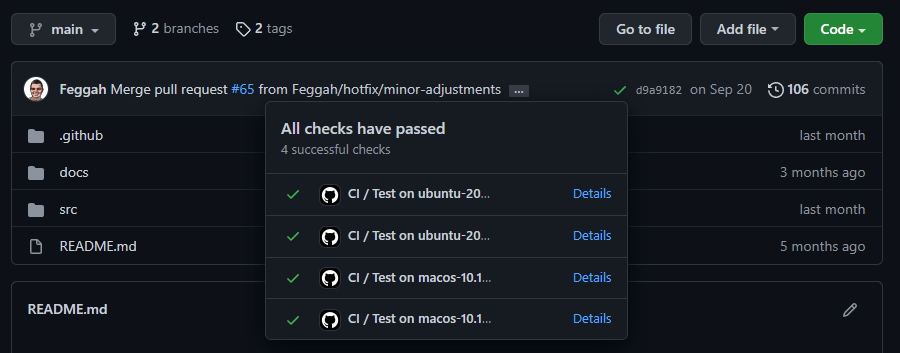
\includegraphics[scale=0.65]{pipeline.png}
  \caption{\textit{Printscreen} dos testes automatizados de \textit{commit} na ramificação principal.}
  \label{fig:pipelineci}
\end{figure}

Durante a implementação do aplicativo, a estrutura de pastas e arquivos reflete diretamente o diagrama de pacotes que foi apresentado na Seção \ref{sec:modelagem}. Existem quatro principais pastas: \textit{data}, \textit{domain}, \textit{presentation} e \textit{shared}.

\begin{figure}[!htb]
  \centering
  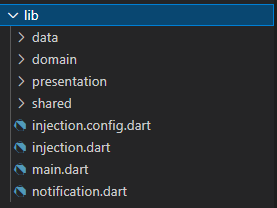
\includegraphics[scale=0.8]{lib-folder-structure.png}
  \caption{\textit{Printscreen} da estrutura de pastas do aplicativo.}
\end{figure}

A pasta \textit{data} contém as implementações dos repositórios, os modelos que são responsáveis pelas conversões entre a entidade interna do aplicativo e a sua representação externa em \textit{frameworks} ou bibliotecas terceiras, e os \textit{datasources}, que são responsáveis por se comunicarem com a \textit{Internet}.

A pasta \textit{domain} contém as entidades da aplicação, as interfaces de repositórios e os casos de uso. Essa pasta é a que deve sofrer menos alterações com o passar do tempo, porque não depende de \textit{frameworks} ou outros fatores que mudam com frequência.

A pasta \textit{presentation} contém as \textit{viewmodels}, a \textit{view} e as rotas do aplicativo. As rotas são utilizadas para fazer a navegação entre as diferentes telas. A \textit{view} contém a definição da interface com os usuários, ou seja, todos os protótipos criados no \textit{Figma} e citados na Seção \ref{sec:uiux}. As \textit{viewmodels} contém a lógica de apresentação das telas, sendo responsável por receber eventos e emitir estados que causam o recarregamento das interfaces para o estado desejado.

A pasta \textit{shared} contém arquivos que são compartilhados entre diversas camadas. Esses arquivos representam as exceções, as possíveis falhas, extensões de bibliotecas terceiras, a implementação de checagem de conectividade com a \textit{Internet} e a interface dos casos de uso.

A visão das pastas expandidas é representada pela \Figura{fig:folders}.

\begin{figure}[!htb]
  \centering
  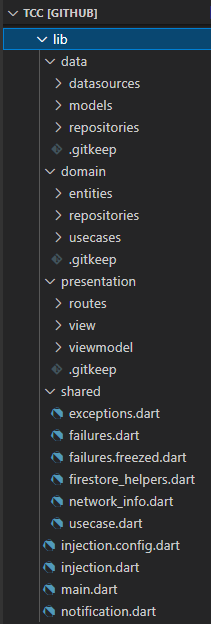
\includegraphics[scale=0.8]{app-folders.png}
  \caption{\textit{Printscreen} da estrutura de pastas expandidas do aplicativo.}
  \label{fig:folders}
\end{figure}

O aplicativo possui uma extensa lista de dependências em bibliotecas de terceiros que foram importadas para cumprir algum objetivo específico. As principais dependências do aplicativo são:

\begin{itemize}
  \item Bibliotecas do \textit{Firebase}, que são alguns \Sigla{\textit{Software Development Kit}}{SDK} que fazem a comunicação com as APIs do \textit{Firebase};
  \item \textit{Flutter\underline{\space}bloc}, que é um pacote para gerenciamento de estados;
  \item \textit{Dartz}, que é uma biblioteca que introduz programação funcional ao \textit{Dart};
  \item \textit{Dio}, que é uma biblioteca para fazer requisições HTTP;
  \item \textit{Get\underline{\space}it}, que é uma biblioteca para utilização do padrão de projeto \textit{Service Locator} para \textit{Dart} e \textit{Flutter}. Esse padrão de projeto é usado para encapsular os processos envolvidos na obtenção de um serviço com uma forte camada de abstração;
  \item \textit{Equatable}, que facilita a comparação de equalidade entre objetos;
  \item \textit{Freezed}, que é um gerador de código para classes imutáveis, introduzindo métodos auxiliares para seus objetos;
  \item \textit{Injectable}, que é um gerador de código para a biblioteca \textit{get\underline{\space}it};
\end{itemize}

Uma das partes mais importantes da implementação do aplicativo é a inversão de dependências, já explicado na subseção \ref{sec:D}. Essa inversão foi implementada utilizando a biblioteca \textit{injectable}.

Para fins de exemplificação, abaixo está exemplificado uma inversão de dependência entre a camada de domínio e a de dados, mais especificamente entre o caso de uso e o repositório.

A dependência do código está do repositório para o caso de uso e o fluxo de dados do caso de uso ao repositório. Para atigir isso, na camada de domínio foi definida a interface do repositório, que neste exemplo é a \textit{ILocationRepository}, representada pela \Figura{fig:locationrepository}.

\begin{figure}[!htb]
  \centering
  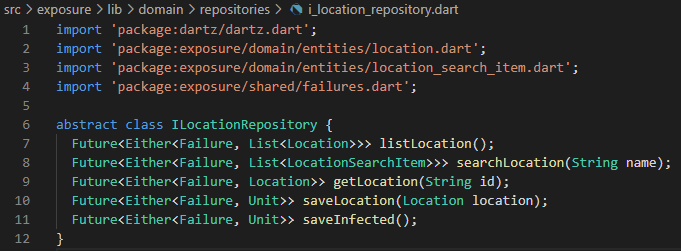
\includegraphics[scale=0.7]{ilocationrepository.png}
  \caption{\textit{Printscreen} da interface \textit{ILocationRepository}.}
  \label{fig:locationrepository}
\end{figure}

Na mesma camada temos o caso de uso \textit{ListLocation}, representado na \Figura{fig:listlocation}, que depende da interface \textit{ILocationRepository}. Essa dependência não fere os princípios da arquitetura limpa porque ambos estão na mesma camada.

\begin{figure}[!htb]
  \centering
  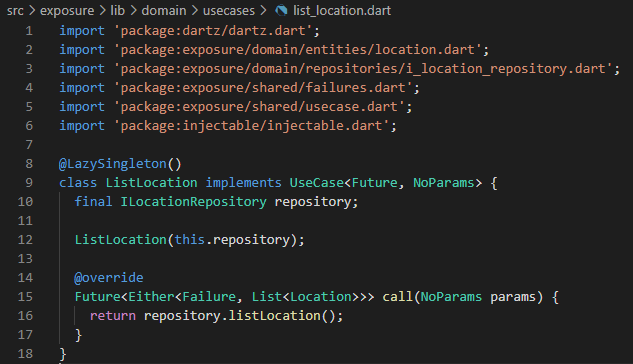
\includegraphics[scale=0.7]{listlocation.png}
  \caption{\textit{Printscreen} do caso de uso \textit{ListLocation}.}
  \label{fig:listlocation}
\end{figure}

Para que a inversão de dependência ocorra, em tempo de execução o atributo \textit{repository} da classe \textit{ListLocation} receberá uma instância da classe \textit{LocationRepositoryImpl} no lugar da \textit{ILocationRepository}. Isso será possível por conta do princípio de Liskov, explicado na subseção \ref{sec:liskov}.

A classe que implementa a interface \textit{ILocationRepository} é chamada de \textit{LocationRepositoryImpl} e está representada na \Figura{fig:locationimpl}. Note que o decorador da classe, que foi importado da biblioteca \textit{injectable}, faz com que as instâncias da classe sejam utilizadas nos atributos do tipo \textit{ILocationRepository}.

\begin{figure}[!htb]
  \centering
  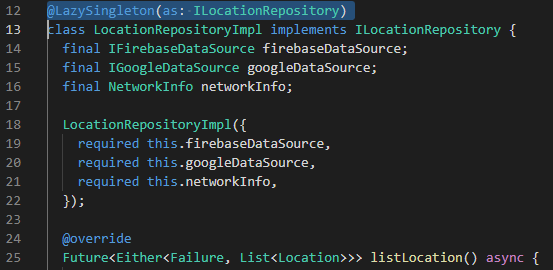
\includegraphics[scale=0.8]{locationimpl.png}
  \caption{\textit{Printscreen} da classe \textit{LocationRepositoryImpl}.}
  \label{fig:locationimpl}
\end{figure}

Esse mesmo modelo foi implementado em todas as fronteiras entre camadas, definindo a interface em uma camada e sua implementação em outra. Com isso, esse princípio da arquitetura limpa foi cumprido em todo aplicativo.

A implementação da \textit{cloud function} que faz a análise do rastreamento entre contatos é responsável por notificar os usuários que forem expostos à alguma doença. A notificação recebida por um dispositivo está exemplificada na \Figura{fig:appnotification}.

\begin{figure}[!htb]
  \centering
  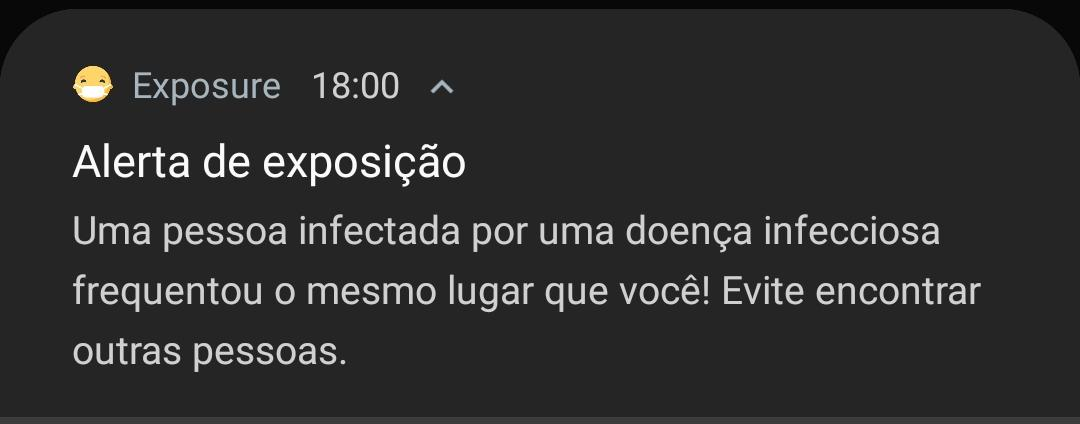
\includegraphics[scale=0.3]{app-notification.jpeg}
  \caption{\textit{Printscreen} da notificação recebida no dispositivo celular.}
  \label{fig:appnotification}
\end{figure}

Um usuário deverá ser notificado se:

\begin{itemize}
  \item A latitude e longitude dos locais salvos são as mesmas. Isso evita falsos positivos em locais com o mesmo nome mas em localizações diferentes. Por exemplo, franquias de uma empresa que estão localizadas em cidades diferentes;
  \item O horário de chegada do usuário é menor que o horário de saída do infectado;
  \item O horário de chegada do infectado é menor que o horário de saída do usuário sendo analisado;
\end{itemize}

Se todas as condições forem verdadeiras, utiliza-se o \textit{fcmToken}, explicado anteriormente na subseção \ref{sec:modelagemdedados}, do documento que representa o usuário para enviar uma notificação ao seu dispositivo. O trecho de código da \Figura{fig:cfscript} referente ao \textit{script} da \textit{cloud function} representa essa análise.

\begin{figure}[!htb]
  \centering
  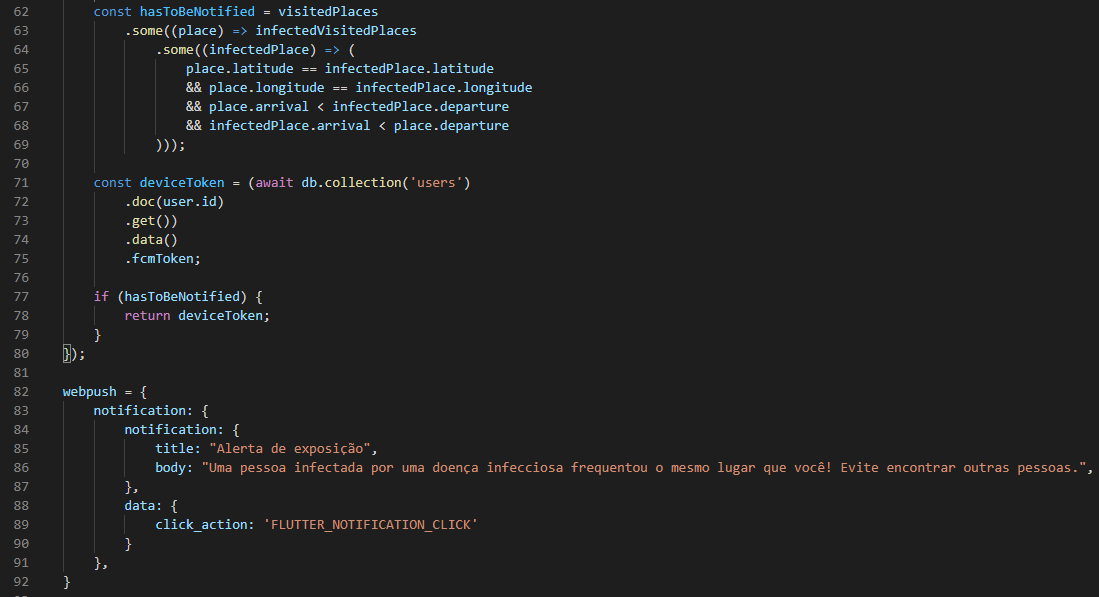
\includegraphics[scale=0.55]{cloudfunction-analysis.png}
  \caption{\textit{Printscreen} do trecho de código da \textit{cloud function}.}
  \label{fig:cfscript}
\end{figure}

As \textit{cloud functions} são definidas a partir de uma sintaxe em que é especificado o evento e o caminho da coleção que serão utilizados para ativá-la. Os possíveis eventos são \textit{OnCreate}, \textit{onUpdate}, \textit{onDelete} e \textit{onWrite}, que respectivamente correspodem aos eventos de criação, alteração, deleção ou todos anteriores.

As duas \textit{cloud functions} desenvolvidas neste trabalho são ativadas a partir de eventos de criação, uma na coleção de locais infectados e outra na subcoleção de locais salvos pelo usuário. A \Figura{fig:cfdeclaration} representa a declaração dessas funções.

\begin{figure}[!htb]
  \centering
  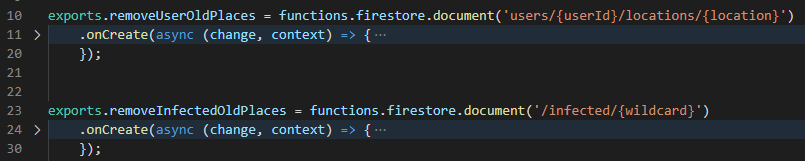
\includegraphics[scale=0.75]{cloudfunction-declaration.png}
  \caption{\textit{Printscreen} da declaração das \textit{cloud functions}.}
  \label{fig:cfdeclaration}
\end{figure}

Em relação a autenticação dos usuários, os IDs são criados aleatoriamente pelo serviço de autenticação do \textit{Firebase}. Como explicado em capítulos anteriores, a autenticação é feita de forma anônima e por conta disso a real identidade do usuário é preservada. Os únicos dados que podem ser extraídos dessa autenticação são a data de criação da conta, a data do último \textit{login} e o seu ID aleatório.

Todo mecanismo de autenticação é feito de forma transparente ao usuário no momento que ele inicia o aplicativo pela primeira vez. Caso o aplicativo seja deletado e instalado novamente, uma nova conta será criada, já que não há mecanismos de associação para definir a real identidade de cada usuário fora do sistema.


\chapter{Infraestrutura}\label{chp:infraestrutura}

Para a realização da solução proposta neste trabalho, recursos de infraestrutura são necessários para que seja possível a execução de rotinas de rastreamento de contatos no servidor, utilização do BD e da comunicação entre o cliente e o servidor. Assim, na Seção \ref{sec:firebase} será explicado o que é e para que serve um serviço de \textit{backend}, quais recursos de infraestrutura serão utilizados e o que são os sistemas de autenticação e o envio de mensagens. Na Seção \ref{sec:firestore} será explicado sobre a solução de BD da plataforma \textit{Firebase} e o que cada entidade dele significa. Por fim, na Seção \ref{sec:cloudfunctions} será explicado o que é a \textit{Cloud Function} e qual será a responsabilidade dela neste projeto.

\section{Serviço de \textit{Backend}}\label{sec:firebase}

A infraestrutura da aplicação será totalmente em nuvem e os principais motivos dessa decisão foram: as faturas de cobrança estão diretamente relacionadas à carga de utilização, e como o escopo deste trabalho é um teste de conclusão de curso, essa carga será baixa; totalmente gerenciado por grandes empresas; boa documentação e facilidade na criação de ambientes.

A nuvem que será utilizada neste trabalho é a \Sigla{\textit{Google Cloud Platform}}{GCP} porque ela entrega serviços que atendem perfeitamente aos requisitos do trabalho, como por exemplo, APIs de busca de locais que utilizam o BD do \textit{Google}.

Neste projeto será utilizado um \Sigla{\textit{Backend-as-a-Service}}{BaaS}, um serviço de \textit{backend} gerenciado por uma empresa. Como a provedora de nuvem escolhida nesse projeto é a GCP, o serviço de BaaS dela se chama \textit{Firebase}.

\textit{Firebase} é uma plataforma digital que tem como objetivo acelerar o processo de desenvolvimento de aplicativos e oferecer serviços que atendam diversos requisitos, como a criação de BDs escaláveis, sistemas de autenticação, sistemas de envio de notificações, dentre outros serviços.

O \textit{Firebase} está diretamente relacionado com a GCP. Todo projeto criado nele também está representado na GCP, a base dos serviços de computação em nuvem da \textit{Google}. A diferença é que o \textit{Firebase} abstrai grande parte da configuração da infraestrutura, gerenciando as configurações necessárias para que os serviços funcionem automaticamente, sem que o usuário precise entender sobre cada detalhe que acontece em segundo plano.

Alguns serviços existem nas duas plataformas, e no fundo são os mesmos, apenas com interfaces de consumo diferentes. Por exemplo, o serviço de \textit{Cloud Functions} pode ser utilizado em ambas plataformas, e quando criado no \textit{Firebase}, também é possível visualizá-lo na interface da GCP.

Porém algumas configurações não são possíveis de serem feitas diretamente pelo \textit{Firebase}. Um exemplo disso é a gestão de identidades, responsável por definir quais permissões cada usuário tem dentro da plataforma e só pode ser configurada pela GCP.

A principal vantagem competitiva do \textit{Firebase} quando comparado a outras plataformas é a alta produtividade que ele traz ao desenvolvimento de aplicativos.

Os serviços do \textit{Firebase} que serão utilizados neste trabalho são o sistema de autenticação, o envio de notificações, o BD e as \textit{Cloud Functions}.

Começando pela autenticação, ela é a peça chave para que os locais visitados pelos usuários sejam salvos em seus respectivos documentos no BD, dando uma experiência personalizada no aplicativo. Essa autenticação pode ser feita de diversas formas diferentes, algumas delas são o \textit{login} utilizando \textit{e-mail} e senha, número de telefone celular, redes sociais e autenticação anônima.

A autenticação anônima, único método de autenticação utilizado pelo aplicativo e explicado com mais detalhes no Capítulo \ref{chp:desenvolvimento}, é criado pelo próprio \textit{Firebase}. Ela é necessária somente para que o aplicativo diferencie os usuários para efetuar o rastreamento, sem precisar de informações pessoais do mesmo.

Outro serviço que será utilizado é o \Sigla{\textit{Firebase Cloud Messaging}}{FCM}, responsável pelo envio de notificações aos usuários que forem possivelmente expostos a alguma doença infecciosa.

O FCM é bastante flexível e possui algumas funcionalidades que atendem diferentes casos de uso. A principal funcionalidade são as formas que a notificação pode ser enviada para o cliente, que são para dispositivos únicos, grupos de dispositivos ou para os dispositivos inscritos em tópicos. 

O envio de notificações deve ser feito de forma automática, para isso, o \textit{Firestore} e as \textit{Cloud Functions} trabalharão em conjunto para que a implementação da lógica do envio de mensagens seja feita com sucesso.

\section{\textit{Firestore}}\label{sec:firestore}

O \textcite{FirestoreDocs} é um BD não relacional orientado a documentos oferecido pelo \textit{Google}. As principais características dele são:

\begin{itemize}
    \item \textit{Serverless}: sem servidor, totalmente gerenciado por tecnologias do Google e com escalonamento automático para atender qualquer carga de requisições;
    \item Mecanismo de consulta avançado: permite a execução de transações com \Sigla{Atomicidade, Consistência, Isolamento e Durabilidade}{ACID} nos dados dos documentos armazenados;
    \item Segurança: integração com a autenticação do \textit{Firebase} para possibilitar controles de acesso de segurança com base na identidade;
    \item Replicação multirregional: redundância de BD em diversos \textit{data centers} espalhados pelo mundo com alta consistência, aumentando a disponibilidade do serviço, mesmo em caso de desastres;
    \item Flexibilidade: o modelo de dados disponibiliza a criação de estruturas hierárquicas flexíveis, onde os dados são armazenados em documentos, e estes organizados em coleções;
    \item Integração: o \textit{Firestore} possui integração perfeita com outros produtos do \textit{Firebase} ou da GCP.
\end{itemize}

O modelo de dados do \textcite{FirestoreDataModel} segue o formato JSON e é estruturado em entidades denominadas documentos e coleções. A \Figura{fig:exemplofirestorejson} apresenta um exemplo dessa estrutura.

\begin{figure}[!htb]
    \centering
    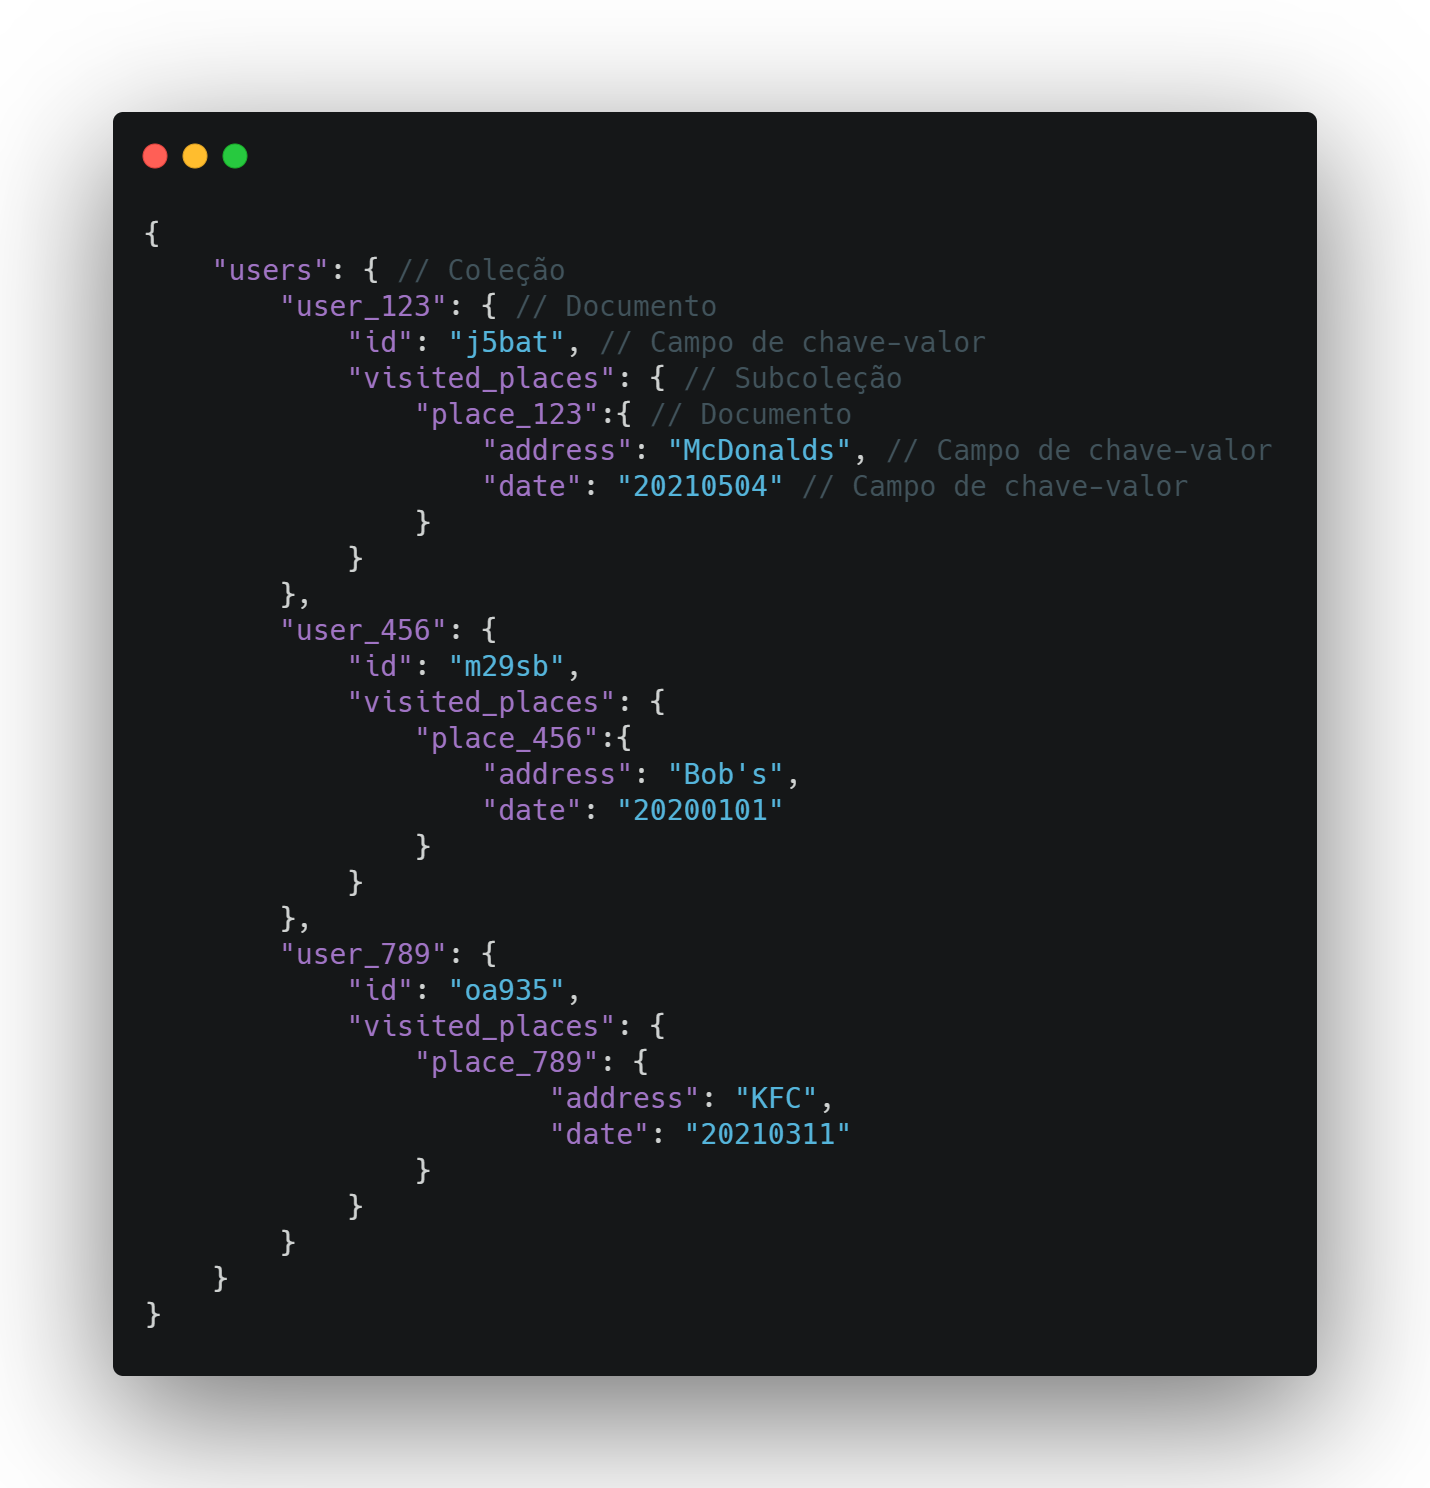
\includegraphics[scale=0.3]{Estrutura Firebase JSON - Carbon Code (estilo Seti).png}
    \caption{Exemplo de estrutura JSON com anotações referentes ao \textit{Firestore}.}
    \label{fig:exemplofirestorejson}
\end{figure}

Documento é a unidade de armazenamento do \textit{Firestore}, com campos mapeados para valores. Esses valores podem ser de diversos tipos: números inteiros, booleanos, \textit{timestamps}, \textit{strings} e até estruturas de dados como listas e mapas.

Cada documento é identificado por um nome e não pode possuir outros documentos criados diretamente dentro dele.

Como o \textit{Firestore} não possui nenhum esquema, o desenvolvedor tem total liberdade sobre quais campos colocar em cada documento e quais tipos de dados esses campos armazenam.

Utilizando os mesmos valores e estrutura da \Figura{fig:exemplofirestorejson}, a \Figura{fig:explicacaodocumentofirestore} representa um exemplo de documento do \textit{Firestore}.

\begin{figure}[!htb]
    \centering
    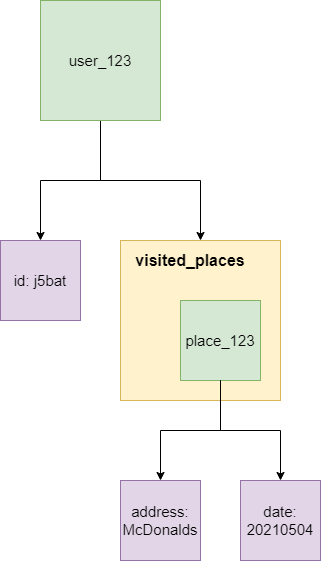
\includegraphics[scale=0.6]{documento-firestore.png}
    \caption{Exemplo de documento do \textit{Firestore}.}
    \label{fig:explicacaodocumentofirestore}
\end{figure}

As coleções são recipientes que armazenam um conjunto de documentos e são referenciadas pelo seu nome, da mesma forma que os documentos.

Os documentos dentro das coleções devem ter identificadores únicos, ou seja, dois documentos diferentes não podem possuir o mesmo nome dentro da mesma coleção. Por conta disso, é comum que os documentos sejam nomeados com o \Sigla{Identificador}{ID} do objeto que ele representa.

É importante ressaltar que coleções não podem armazenar dados diretamente, apenas através de documentos. Cada entidade possui responsabilidades específicas. Por conta disso, para criar uma estrutura hierárquica no \textit{Firestore}, as coleções armazenam exclusivamente documentos, e os documentos, além dos campos chaves-valor, podem armazenar subcoleções - que possuem as mesmas características de uma coleção.

Para melhor visualização da estrutura hierárquica do \textit{Firestore}, a estrutura da \Figura{fig:exemplofirestorejson} está representada na \Figura{fig:explicacaofirestorecompleto}.

\begin{figure}[!htb]
    \centering
    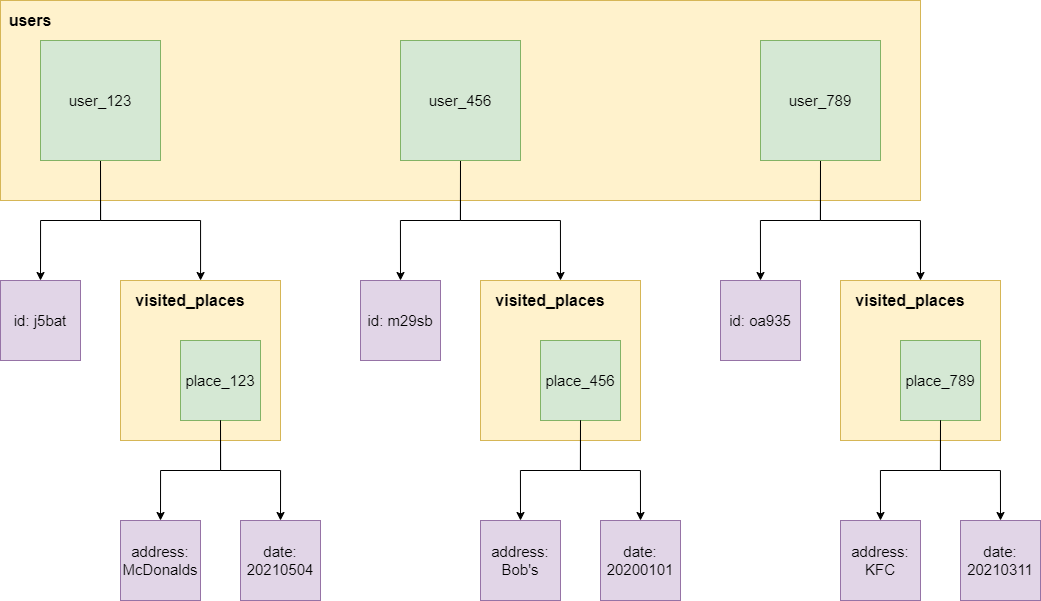
\includegraphics[scale=0.43]{Estrutura Firestore.png}
    \caption{Exemplo de estrutura hierárquica do \textit{Firestore}}
    \label{fig:explicacaofirestorecompleto}
\end{figure}

\section{\textit{Cloud Functions}}\label{sec:cloudfunctions}

A \textit{Cloud Function} é o produto de função como serviço para criar aplicações com base em eventos, disponibilizado pelas plataformas \textit{Firebase} e GCP. Ela é uma maneira de ampliar o comportamento de um aplicativo e integrar com outros recursos disponíveis na plataforma por meio da adição de código no servidor. Com base nisso, ela serve como camada conectiva, disponibilizando a construção de lógicas entre os serviços da plataforma por meio da detecção e da resposta a eventos.

No caso de uso deste trabalho, a \textit{Cloud Function} consome os eventos de escrita em coleções específicas no \textit{Firestore}, tratando-os através da execução do trecho de código implementado na função.


\chapter{Conclusões}\label{chp:conclusoes}

Este trabalho apresentou uma abordagem automatizada de rastreamento de contatos. Foi proposta uma solução baseada em um aplicativo de dispositivos móveis, disponível para a maioria dos sistemas operacionais, permitindo a utilização do produto por grande parte da população.

Por meio de testes com diferentes dispositivos foi validado que a solução está funcional e possui a capacidade de notificar as pessoas possivelmente expostas à alguma doença infecciosa.

Com isso, o aplicativo conseguiu resolver o problema manual que foi relatado no Capítulo \ref{chp:Introducao}, transformando o alto número de pessoas para efetuar o rastreamento de contatos com cada infectado em uma solução digital automatizada. A única necessidade manual é por parte dos usuários, que devem fazer os \textit{check-ins} e declararem no aplicativo quando forem infectados, para que as rotinas de análise sejam ativadas.

\section{Trabalhos futuros}
As sugestões de trabalhos futuros baseiam-se na implementação de mais funcionalidades ao aplicativo, destacando-se:
\begin{itemize}
    \item A substituição da utilização de \textit{check-ins} por \textit{Bluetooth}. Essa solução faria com que o rastreamento se tornasse totalmente automático, porque remove a necessidade do usuário fazer os \textit{check-ins} de suas visitas, e pode ser cumprida através do desenvolvimento de uma biblioteca própria ou da comunidade com as funcionalidades necessárias do \textit{Bluetooth}.
    \item Adicionar suporte para que o usuário consiga deletar os dados salvos no aplicativo, isso significa dar suporte a deleção dos locais salvos e a opção de deleção da conta;
    \item Construção de um painel administrativo, onde haverão gráficos de calor que extraem informações do BD, para que autoridades públicas possam tomar medidas de prevenção em locais onde estão sendo transmitidas doenças infecciosas em uma taxa crítica. Esse painel deve ser acessado somente por pessoas específicas e seria uma extensão total do sistema, necessitando outros mecanismos de autenticação, telas, bancos de dados e funcionalidades;
\end{itemize}


% Comandos para incluir as referências bibliográficas
% Define espaçamento simples em cada referência
\begin{singlespacing}

% Adiciona uma linha em branco entre duas referências
\setlength\bibitemsep{10pt}   

\printbibliography[heading=bibintoc, % Adiciona no sumário
                   title={Referências bibliográficas} % Nome do Capítulo
                  ]
\end{singlespacing}

% Os anexos, se houver, vêm depois das referências:
%\appendix

% O comando a seguir inclui o arquivo apendices.tex
% que contém os apêndices. Observe o comando \appendix
% na linha anterior
% Detalhe: não precisa incluir a extensão .tex
%%\chapter{Primeiro Apêndice}
% O comando a seguir gera um "dummy text". 
% Elimine-o quando escrever sua dissertação.
%\lipsum[9]

%\chapter{Segundo  Apêndice}
% O comando a seguir gera um "dummy text". 
% Elimine-o quando escrever sua dissertação.
%\lipsum[10]

%
\end{document}